\chapter{Search for invisibly decaying VBF produced Higgs bosons in Run 1 prompt data}
\label{chap:prompt}
%Introduction to selection and challenges of jets+met, e.g. trigger, \ac{QCD}
As described in \ChapterRef{chap:theory}, searches for invisible Higgs boson decays are well motivated by their sensitivity to new physics, such as \ac{DM}. Because \BRinv of an \ac{SM} 125 \GeV Higgs boson is very small, any evidence for invisible Higgs boson decays at the \LHC would be evidence for physics beyond the \ac{SM}. This chapter describes the search for invisible Higgs boson decays using data taken by CMS in 2012 which was promptly reconstructed. A dedicated trigger was developed specifically for this analysis. The total integrated luminosity collected with this trigger that was certified for use in physics analyses was 19.5\,\invfb~\cite{CMS-PAS-LUM-13-001}. The analysis was published in \ReferenceRef{Chatrchyan:2014tja}.

\section{Event selection}
\label{sec:promptsel}
%describe backgrounds and motivate selection
Signal events are expected to have two jets with a characteristic \ac{VBF} topology and a large amount of \MET. Several background processes, with significantly higher cross-sections than the signal process, can also produce events containing these objects. It is therefore necessary to design selection criteria, known as ``cuts'', to remove as many of these background events from the analysis as possible, whilst retaining the maximum number of signal events.

The most significant of these background processes is the production of a vector boson in association with jets, ``V+jets''. Leptonic decays of \PW bosons and \PZ boson decays to neutrinos both produce \MET and, due to the approximately 1000 times higher cross-section for vector boson production than Higgs boson production, in many events the associated jets have a \ac{VBF}-like topology~\cite{CMSSMPPublic}. V+jets backgrounds with a \PW (\PZ) are referred to as ``\PW(\PZ)+jets''.
A further background process that can produce significant numbers of \ac{VBF}-like jets due to its very large cross-section is \ac{QCD} production of multiple jets (``\ac{QCD} multijets'' or simply ``\ac{QCD}''). Whilst these multijet events have very little \MET from real invisible particles, it is possible for significant ``fake'' \MET to be caused by mismeasurement of the jets. The production of two vector bosons or top quarks can also lead to two jets and real \MET, although they have much lower cross-sections than the other background processes and their contribution is not as significant. %relative cross-section

%trigger requirements and design
\subsection{Trigger}
\label{sec:prompttrig}
The trigger requirements can be viewed as the first stage of the event selection. Their primary role is to reduce the rate of events that must be recorded by the detector, whilst retaining the maximum number of signal events. As described in \SectionRef{sec:triggers}, the decision whether to keep an event must be made very rapidly and, as a result, the object reconstruction algorithms used are less sophisticated, and the granularity of the information available from the CMS subdetectors is worse than those offline. The trigger criteria have therefore been chosen to be as loose as possible whilst achieving the required rate reduction.

As it is the key variable which indicates the presence of invisible particles, all events passing the trigger are required to have significant \MET. To pass the \ac{L1} trigger selection events are required to have \MET$>40$ \GeV. The \ac{HLT} selection also requires that events have \METnoMU$>65$\GeV. The use of \METnoMU at trigger level ensures that events that are needed for the control regions used in the background estimation techniques described in \SectionRef{sec:promptbkg} are not rejected. In addition to this \METnoMU requirement events must have at least one pair of jets which is \ac{VBF}-like to pass the \ac{HLT} selection. The \ac{VBF}-like requirements on the jets consist of requiring their $\eta$ separation, \detajj, to be greater than 3.5, that they are in opposite forward/backward halves of the detector and that they have high invariant mass, $\Mjj>800 \GeV$. All of these jet requirements are motivated by the lack of colour connection between the jets in \ac{VBF} events leading to large angular separations between the two jets, as described in \SectionRef{sec:higprod}. The requirement that jets be in opposite forward/backward halves of the detector is made almost redundant by the \detajj cut, however it is a fast requirement to compute and is applied early in the list of trigger requirements and thus decreases the resource usage of the trigger. Not requiring that the \ac{VBF}-like pair of jets also be the two highest \pt jets reduces inefficiencies caused by different \pt orderings in jets reconstructed by the trigger and by the offline reconstruction.

The efficiency for events passing both the prompt analysis trigger and the two triggers used for the parked data analysis, described in \ChapterRef{chap:parked} as a function of their values of several offline variables, measured in single muon data collected using an uncorrelated trigger, is shown in Figs.~\ref{fig:prompttrigplots} and \ref{fig:prompttrigplots2}. The events used in the trigger efficiency measurement are required to pass the following cuts:
\begin{equation}
  \label{eq:prompttrigstudycuts}
  \Mjj>1100 \GeV, \METnoMU>130 \GeV, \mathrm{leading\,2\,jets'\,} \pt>50 \GeV, \detajj>4.2,\eta_{j1}\cdot\eta_{j2}<0.
\end{equation}
In each measurement the cut on the variable being studied is removed. The measured trigger efficiency is applied as an event-by-event weight to all \ac{MC} samples.

%trigger efficiency plots from trigeff310314
\begin{figure}
  \subfloat[]{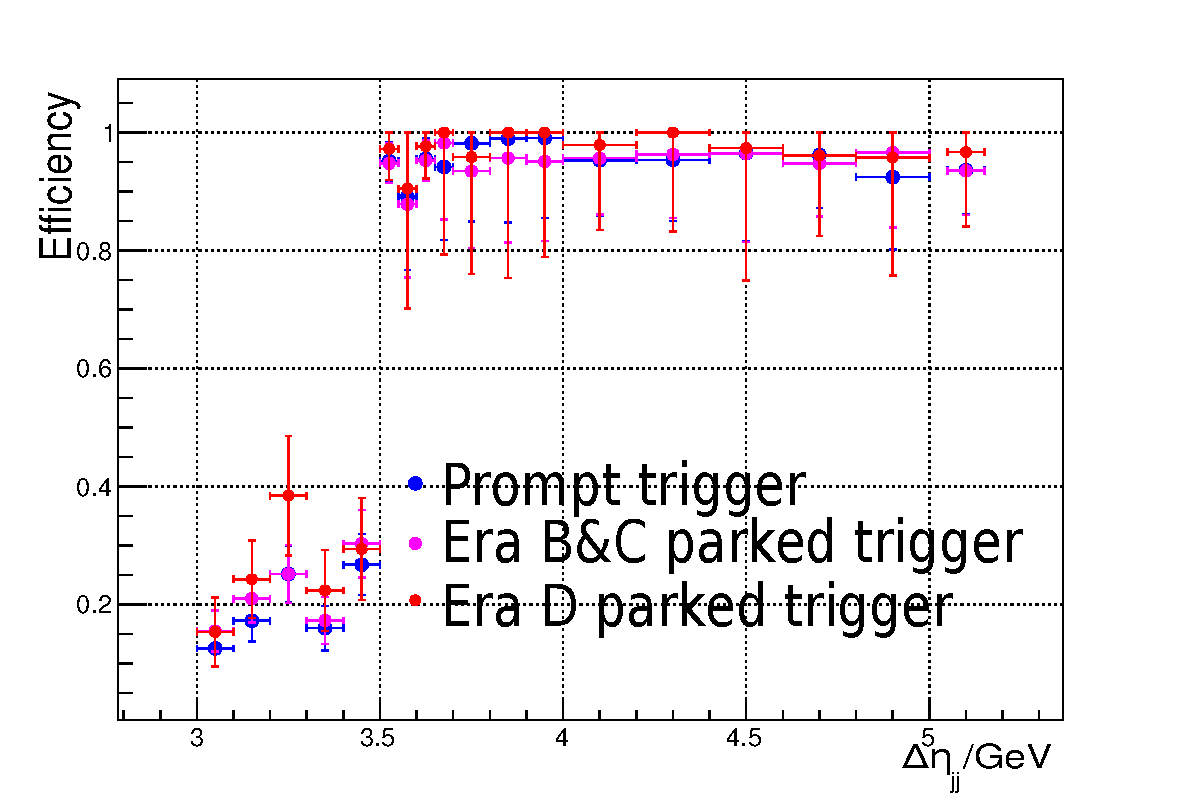
\includegraphics[width=.65\largefigwidth]{plots/prompt/trigeffplots_hltonly/detaefficiency.pdf}}
  \subfloat[]{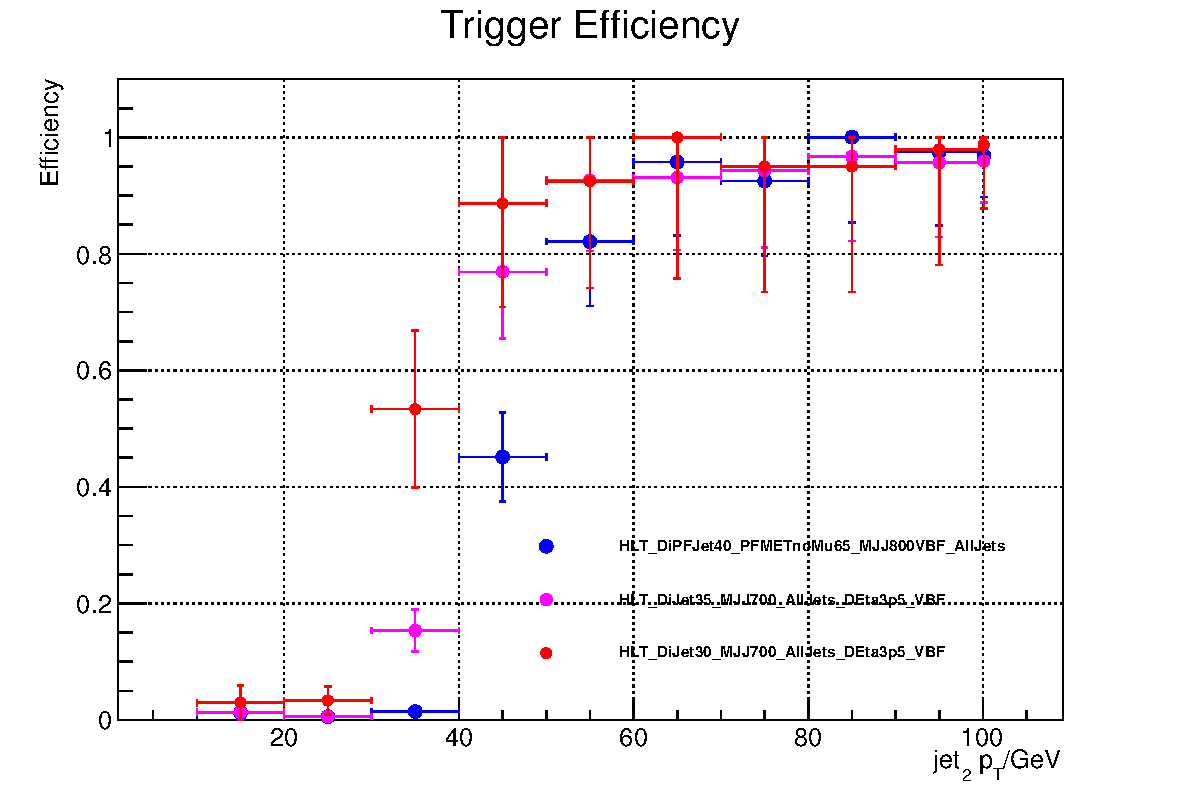
\includegraphics[width=.65\largefigwidth]{plots/prompt/trigeffplots_hltonly/j2ptefficiency.pdf}}

  \subfloat[]{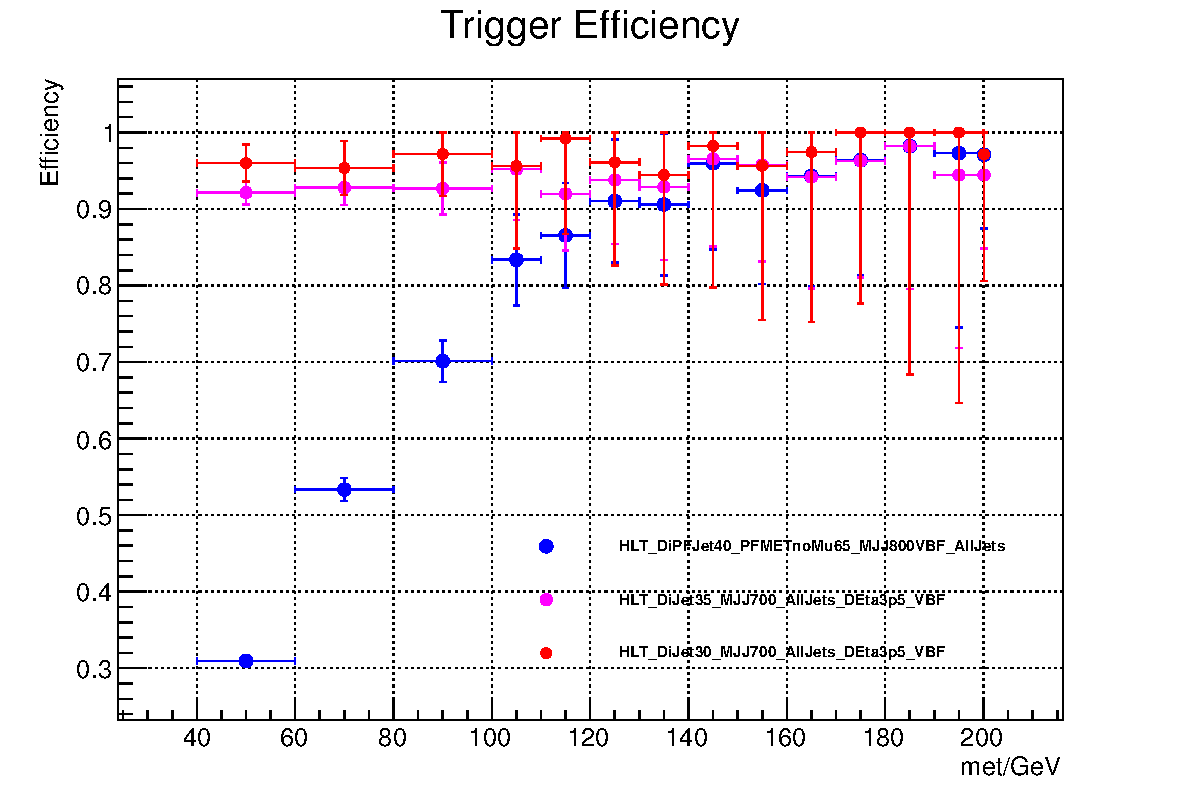
\includegraphics[width=.65\largefigwidth]{plots/prompt/trigeffplots_hltonly/metefficiency.pdf}}
  \subfloat[]{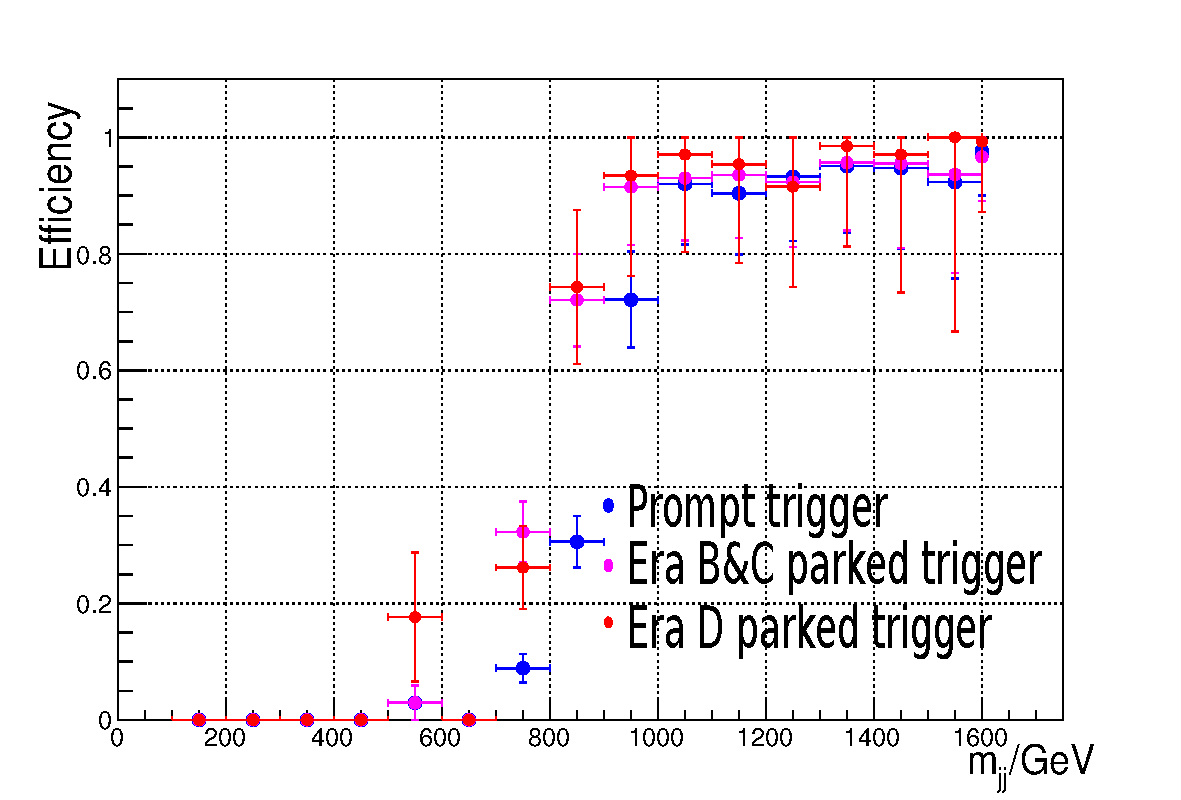
\includegraphics[width=.65\largefigwidth]{plots/prompt/trigeffplots_hltonly/mjjefficiency.pdf}}
  \caption{The efficiency of the HLT requirements used in the prompt (blue) and parked (purple and red) data analyses as a function of the values of several offline variables, measured in a sample of events recorded on a single-muon trigger. (a) Efficiency as a function of offline \detajj, (b) efficiency as a function of sub-leading jet \pt, (c) efficiency as a function of offline \METnoMU, (d) efficiency as a function of \Mjj.}
  \label{fig:prompttrigplots}
\end{figure}

\begin{figure}
  \subfloat[]{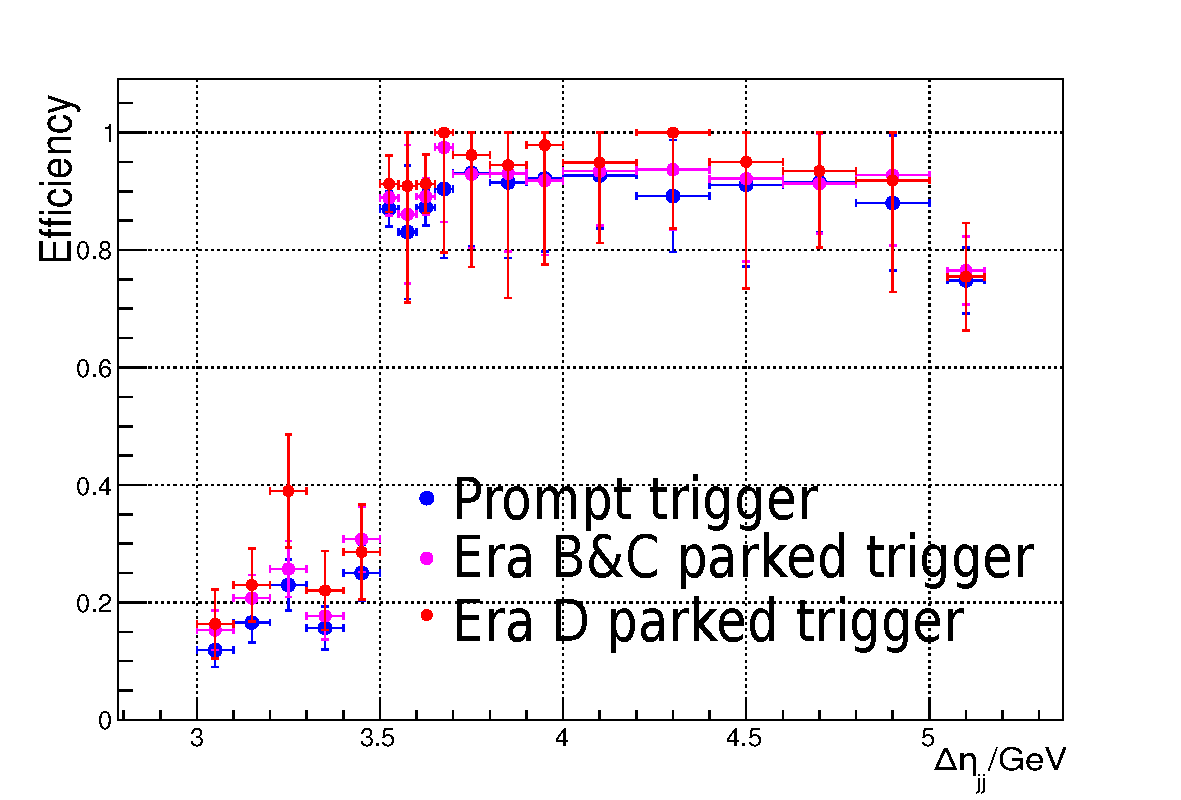
\includegraphics[width=.65\largefigwidth]{plots/prompt/trigeffplots_nol1cut/detaefficiency.pdf}}
  \subfloat[]{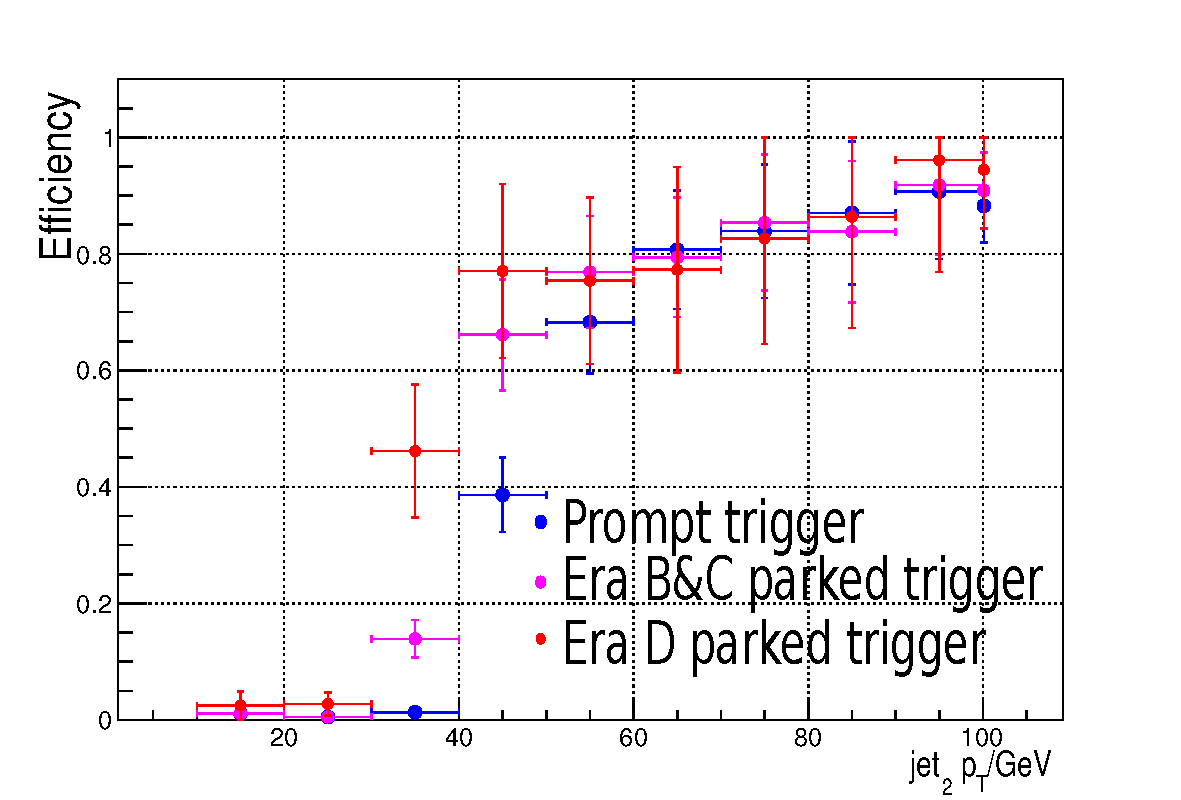
\includegraphics[width=.65\largefigwidth]{plots/prompt/trigeffplots_nol1cut/j2ptefficiency.pdf}}

  \subfloat[]{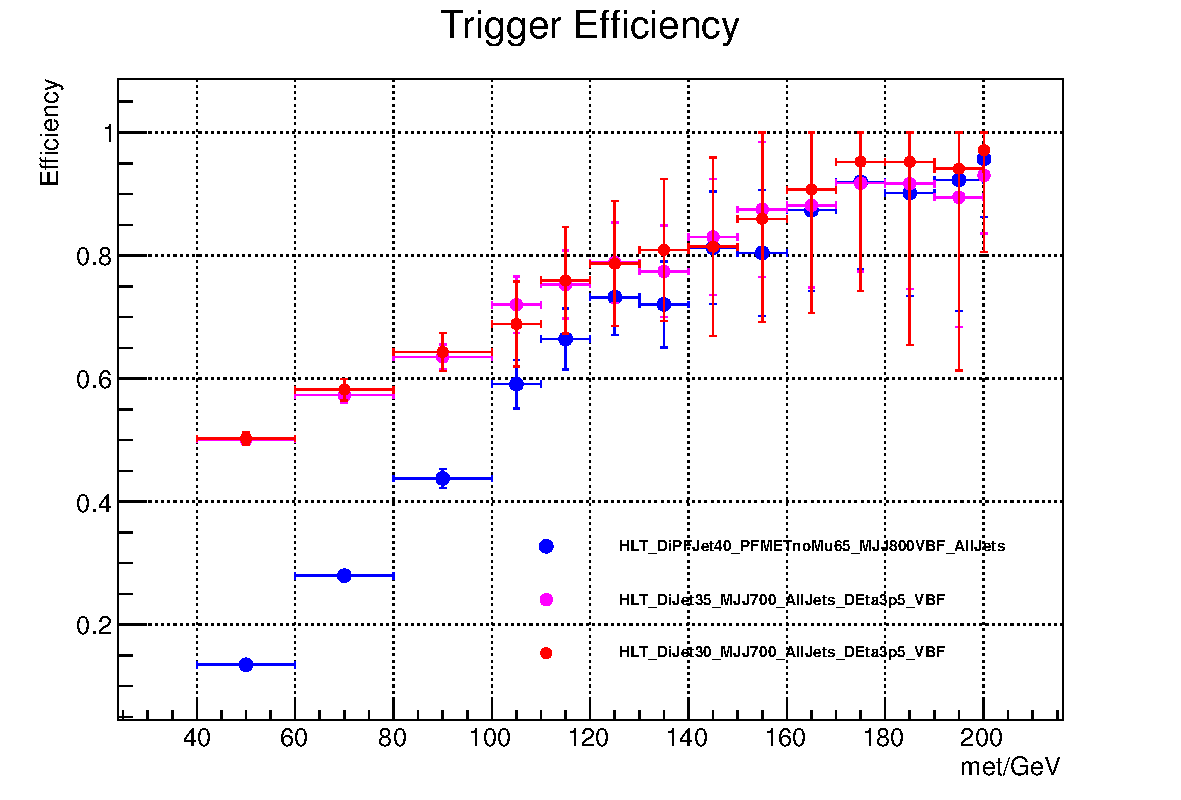
\includegraphics[width=.65\largefigwidth]{plots/prompt/trigeffplots_nol1cut/metefficiency.pdf}}
  \subfloat[]{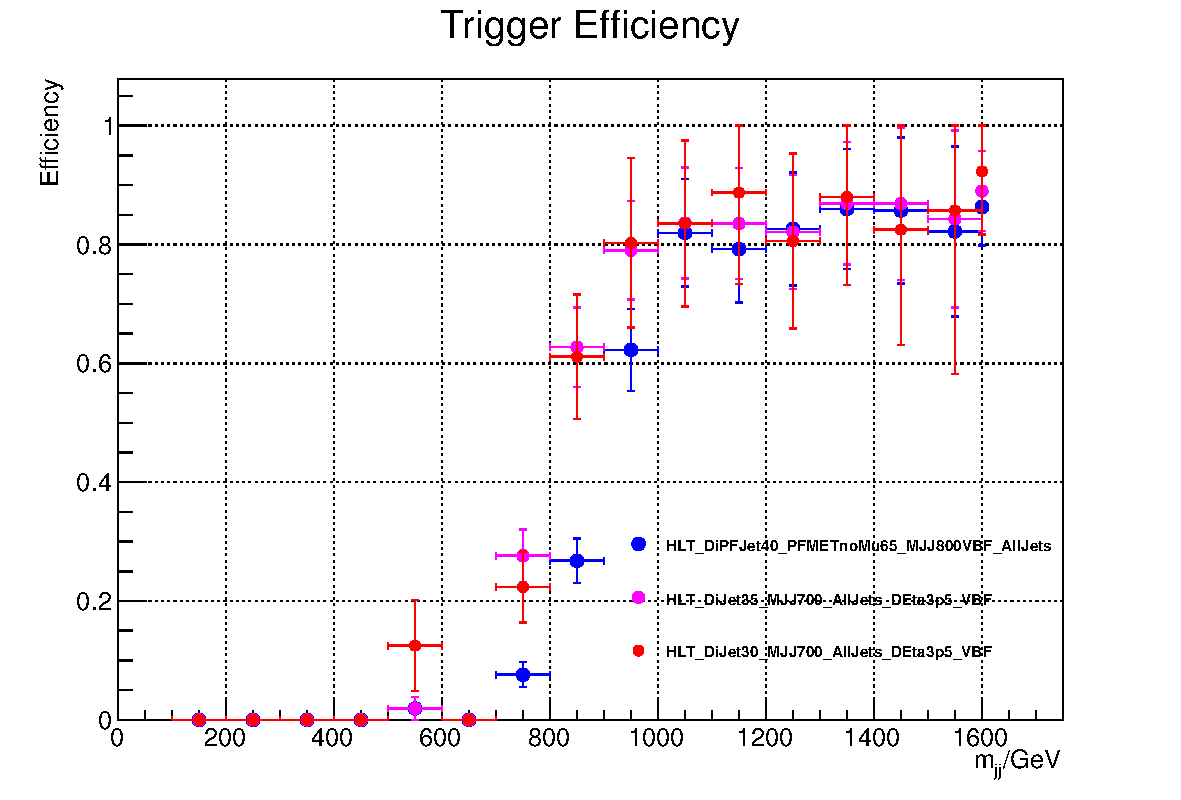
\includegraphics[width=.65\largefigwidth]{plots/prompt/trigeffplots_nol1cut/mjjefficiency.pdf}}
  \caption{The combined efficiency of the HLT and L1 trigger requirements used in the prompt (blue) and parked (purple and red) data analyses as a function of the values of several offline variables, measured in a sample of events recorded on a single-muon trigger. (a) Efficiency as a function of offline \detajj, (b) efficiency as a function of sub-leading jet \pt, (c) efficiency as a function of offline \METnoMU, (d) efficiency as a function of \Mjj.}
  \label{fig:prompttrigplots2}
\end{figure}

\subsection{Offline selection}
\label{sec:promptofflinesel}
%selection and motivation
The offline selection is chosen for three reasons. Firstly, the reconstruction algorithms for some objects are only well validated for certain values of \pt and $\eta$. This consideration decides the $\pt$ thresholds for jets and leptons to be used. Secondly, as can be seen from \FigureRef{fig:prompttrigplots}, the values of the offline variables where the trigger becomes fully efficient are in some cases much higher than the online cut. Because the variables used in the trigger are highly correlated, and the measurements of trigger efficiency made do not take this into account, the offline cuts on all variables used in the trigger were chosen such that the trigger efficiency for the variable at that point is greater than 95\%. Finally, some of the cuts imposed aim to reduce the contribution from background processes, which improves the signal to background ratio in the resulting region, and thus the expected limit on \BRinv.

The specific set of offline selection cuts chosen begins by requiring that events have no veto muons or electrons, as defined in Sections \ref{sec:electrons} and \ref{sec:muons}. Signal events are not expected to contain leptons, while background events are, so this lepton veto reduces the background from \PW and \PZ boson decays and also from top quarks without removing signal events. The two highest \pt jets in the event are then identified as the VBF tag pair, and tighter versions of the trigger selection, motivated by the trigger efficiency considerations described above, are then applied. Specifically, the tag jets are required to be in opposite forward/backward halves of the detector, to both have \pt$>50$ \GeV to have $\Mjj>1100$ \GeV and $\detajj>4.2$. Again due to trigger efficiency considerations, \METnoMU is required to be greater than 130 \GeV.  Because events with veto muons have been removed by the lepton veto, \METnoMU in this region is identical to \MET. However, it is important for background estimation methods that \METnoMU and not \MET is used.

As well as the trigger-based selection, further cuts are made to reduce the \ac{QCD} background to a level much lower than the V+jets backgrounds. The two tag jets are required to have an azimuthal separation, $\dphijj<1.0$, since multijet events with \MET due to mismeasurement are most likely to have their jets back-to-back in the detector, i.e. with $\dphijj=\pi$. Events where there are any jets with \pt$>30$ \GeV between the two tag jets in $\eta$ are also vetoed. This \ac{CJV} is motivated by the lack of colour connection, described in \SectionRef{sec:higprod}, between the quarks in VBF production that makes the presence of such jets unlikely in genuine signal events. The region of phase space remaining after all these cuts have been applied is called the signal region.

Finally, the values of the cuts are optimised to provide the best expected limit on \BRinv\, for a 125 \GeV Higgs boson, which is calculated using the method described in \SectionRef{sec:stats} using the same background estimation and systematic uncertainties as the final analysis (as described in Sections~\ref{sec:promptbkg} and \ref{sec:promptsyst} respectively). For the tag jet \pt and \METnoMU, no improvement in the expected limit is seen by tightening the cut, so the requirement is set at the 95\% efficiency point of the trigger. The distributions and cut values for several of the other variables used are shown in \FigureRef{fig:promptcontrolplots}. The full selection gives an efficiency of $(6.8\pm 0.3)\times 10^{-3}$ for selecting events from invisible decays of a VBF-produced 125 \GeV Higgs boson, measured using \ac{MC}.  

%discriminating variable plots from HIG-13-030
\begin{figure}
  \subfloat[]{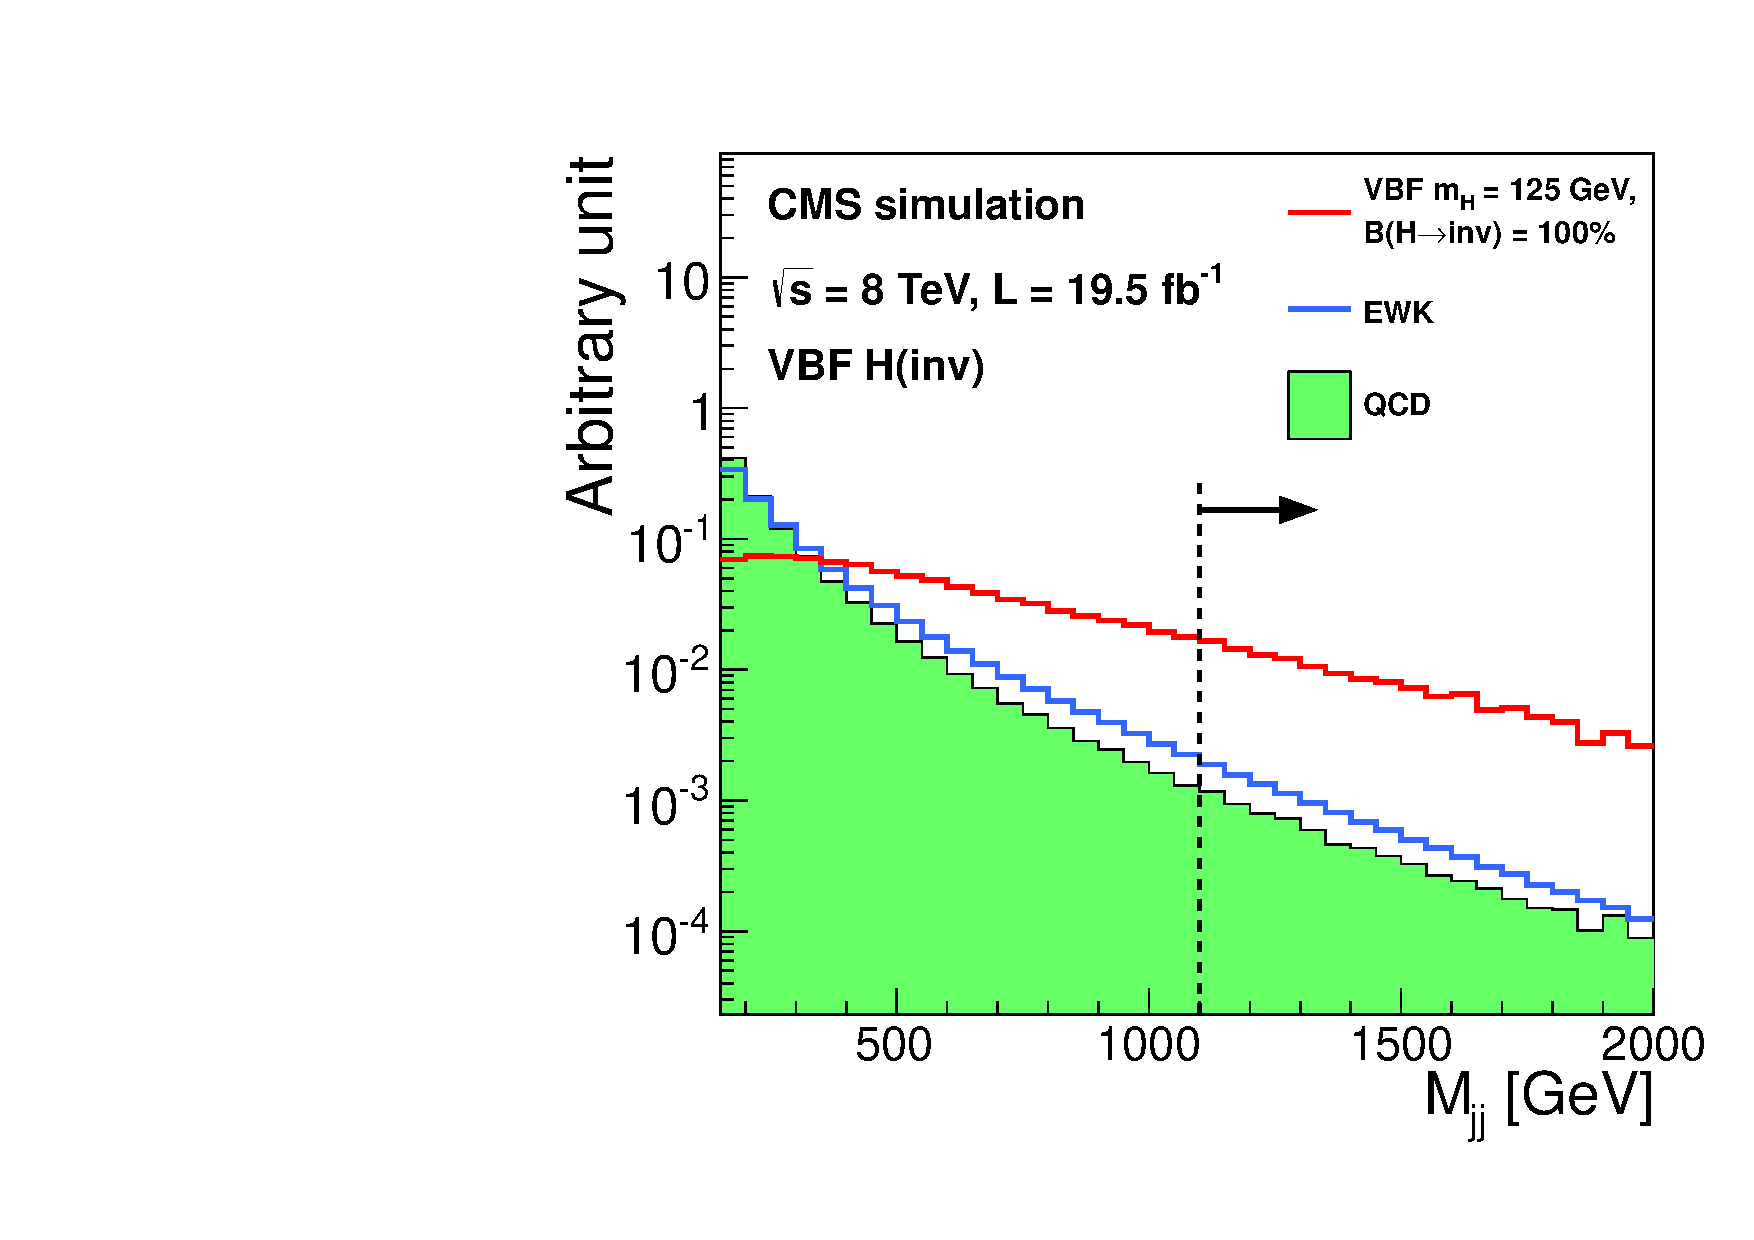
\includegraphics[width=.65\largefigwidth]{plots/prompt/VBF-Dijet-M.pdf}}
  \subfloat[]{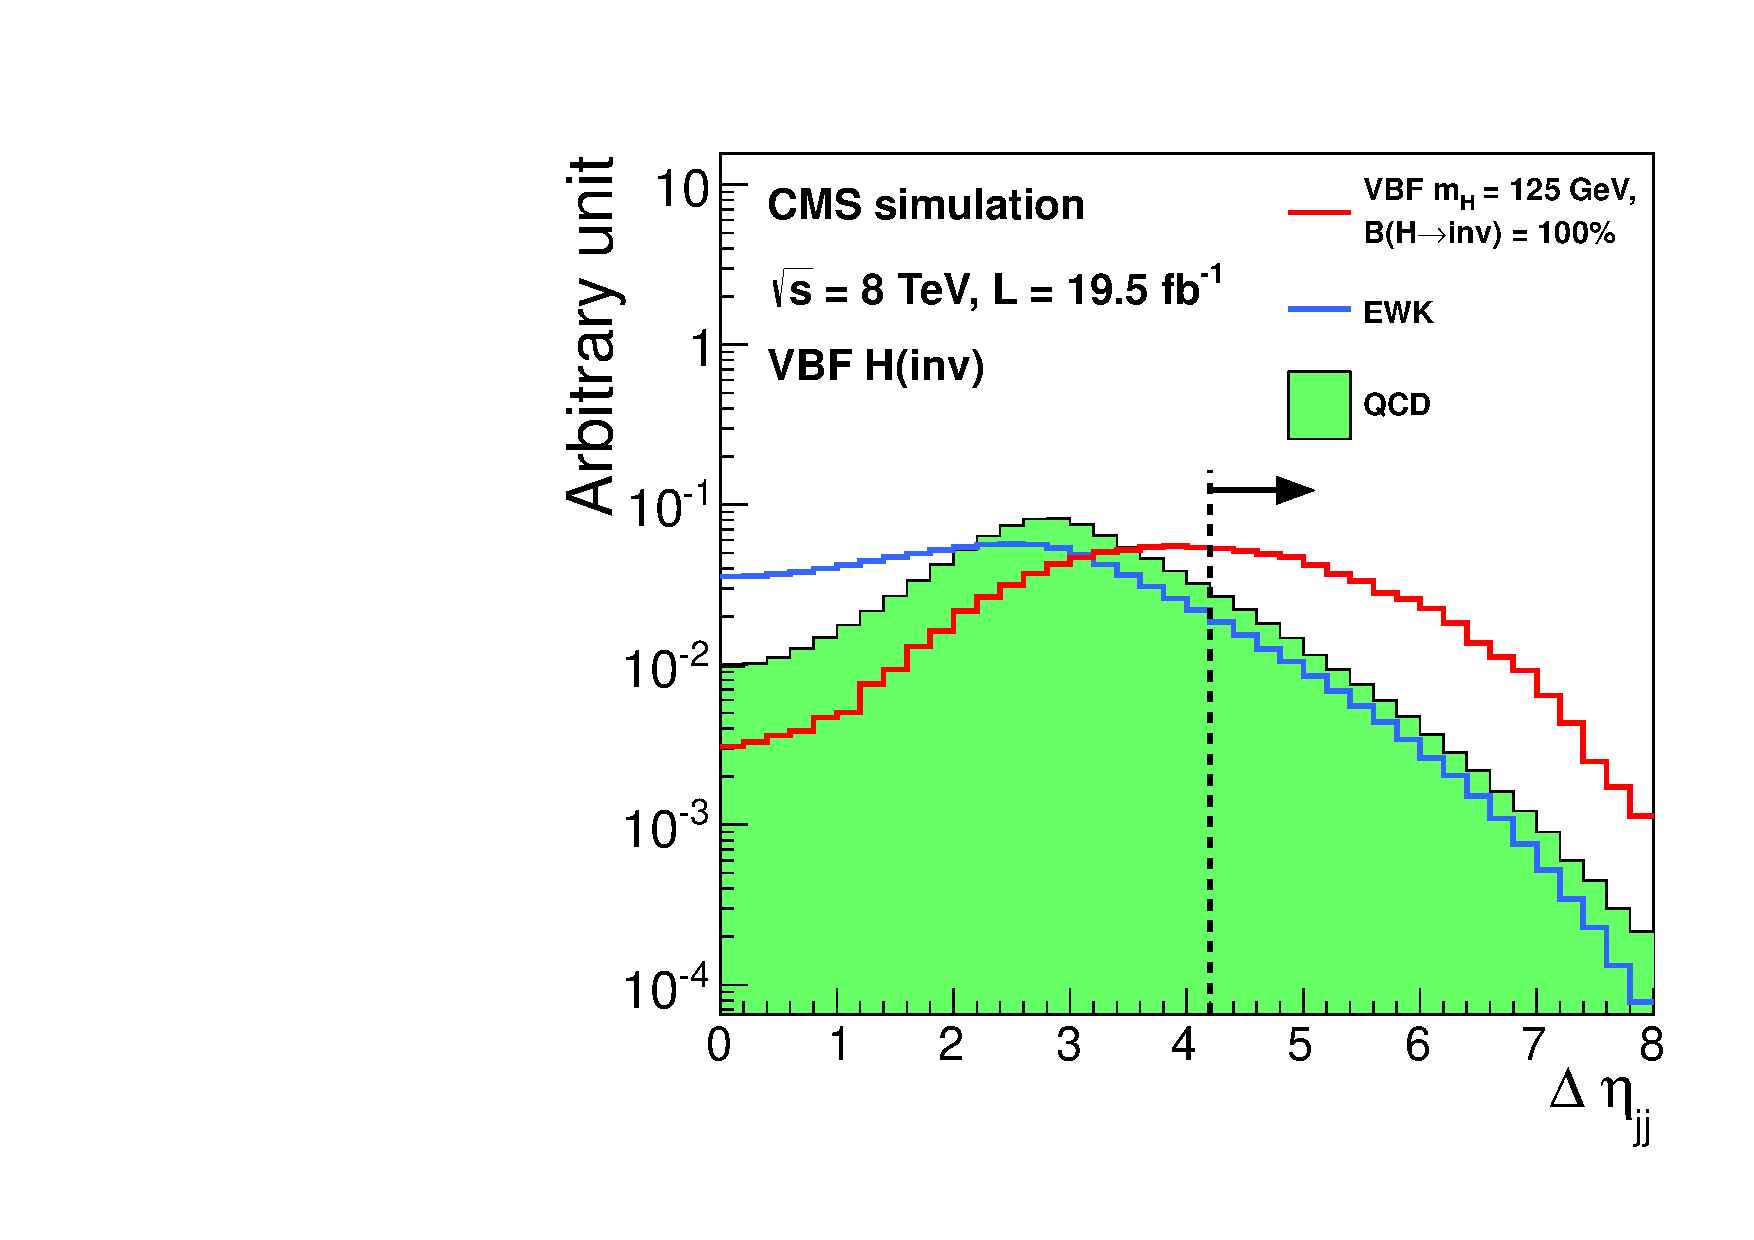
\includegraphics[width=.65\largefigwidth]{plots/prompt/VBF-Dijet-DEta.pdf}}

  \subfloat[]{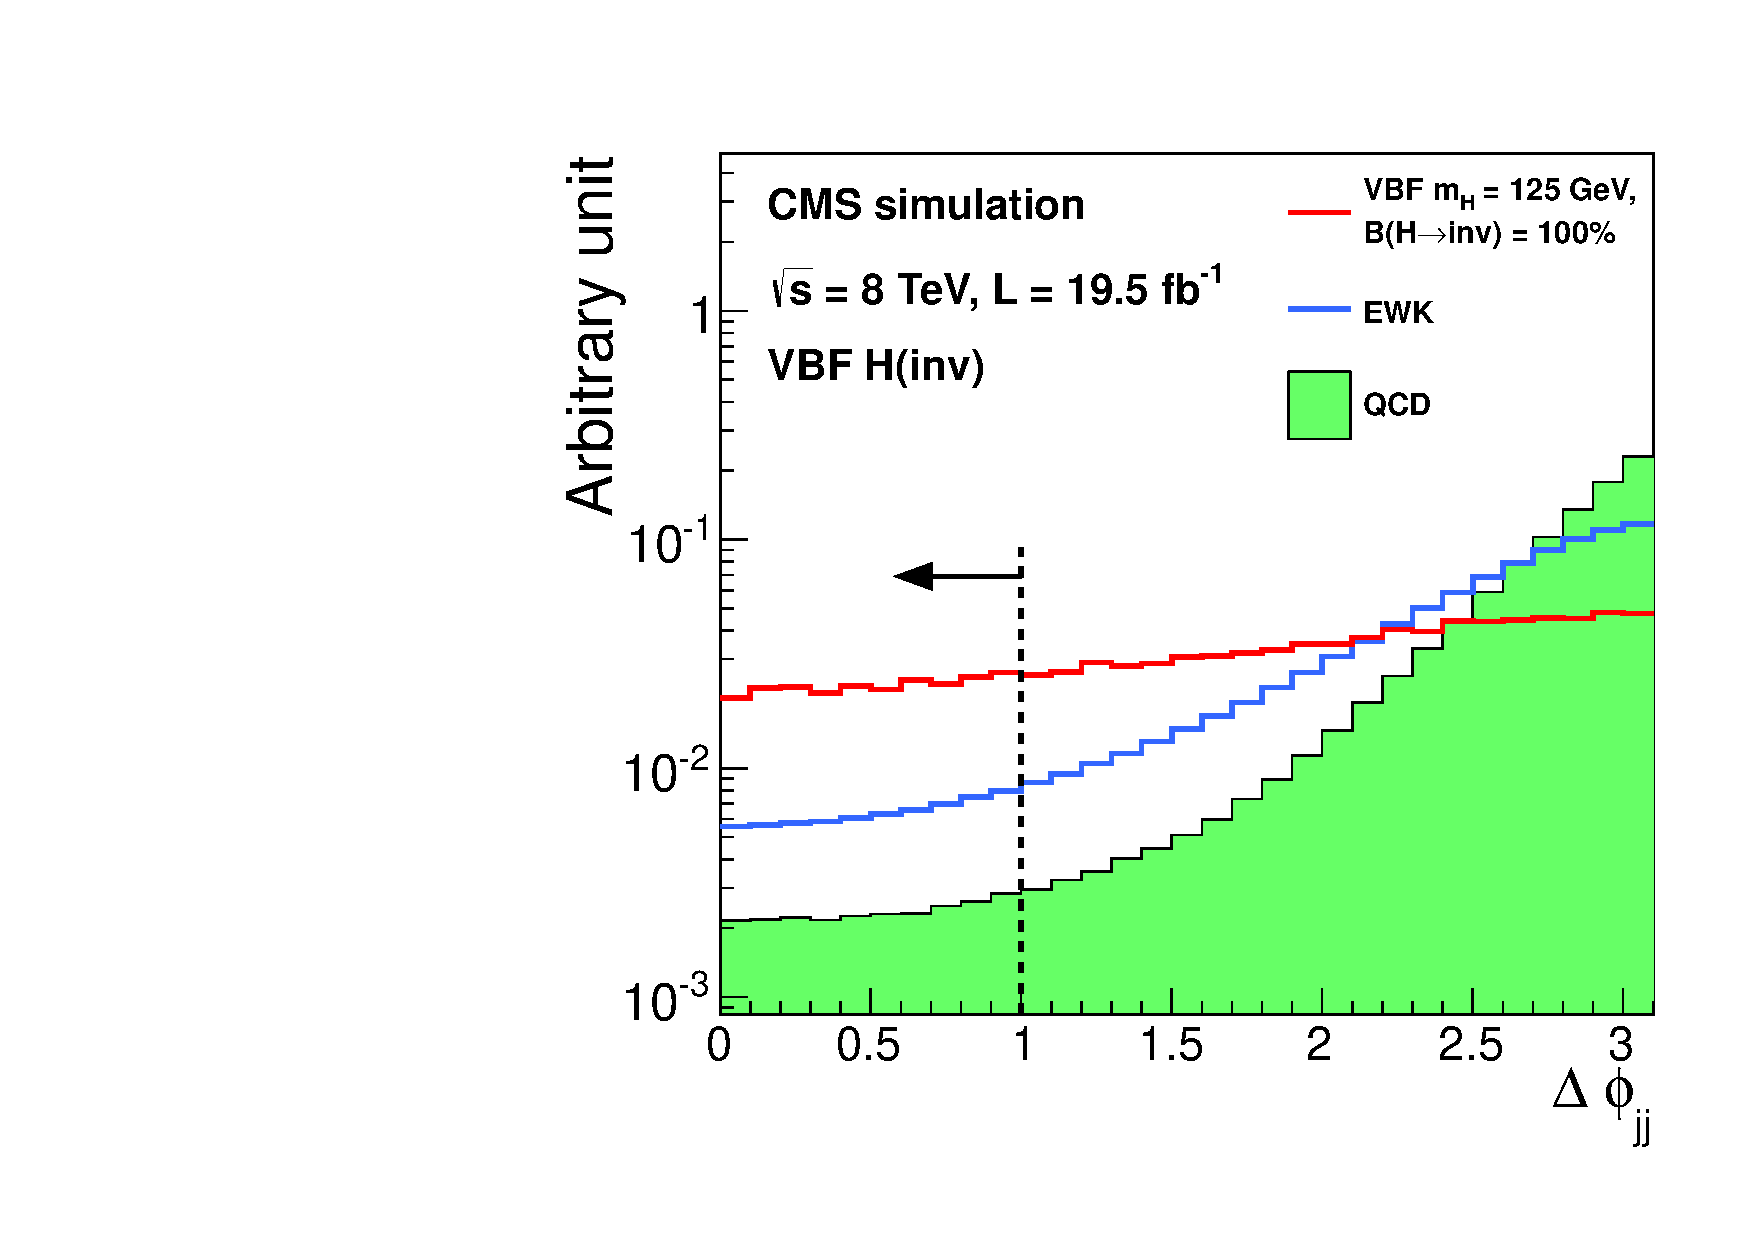
\includegraphics[width=.65\largefigwidth]{plots/prompt/VBF-Dijet-DPhi.pdf}}
  \subfloat[]{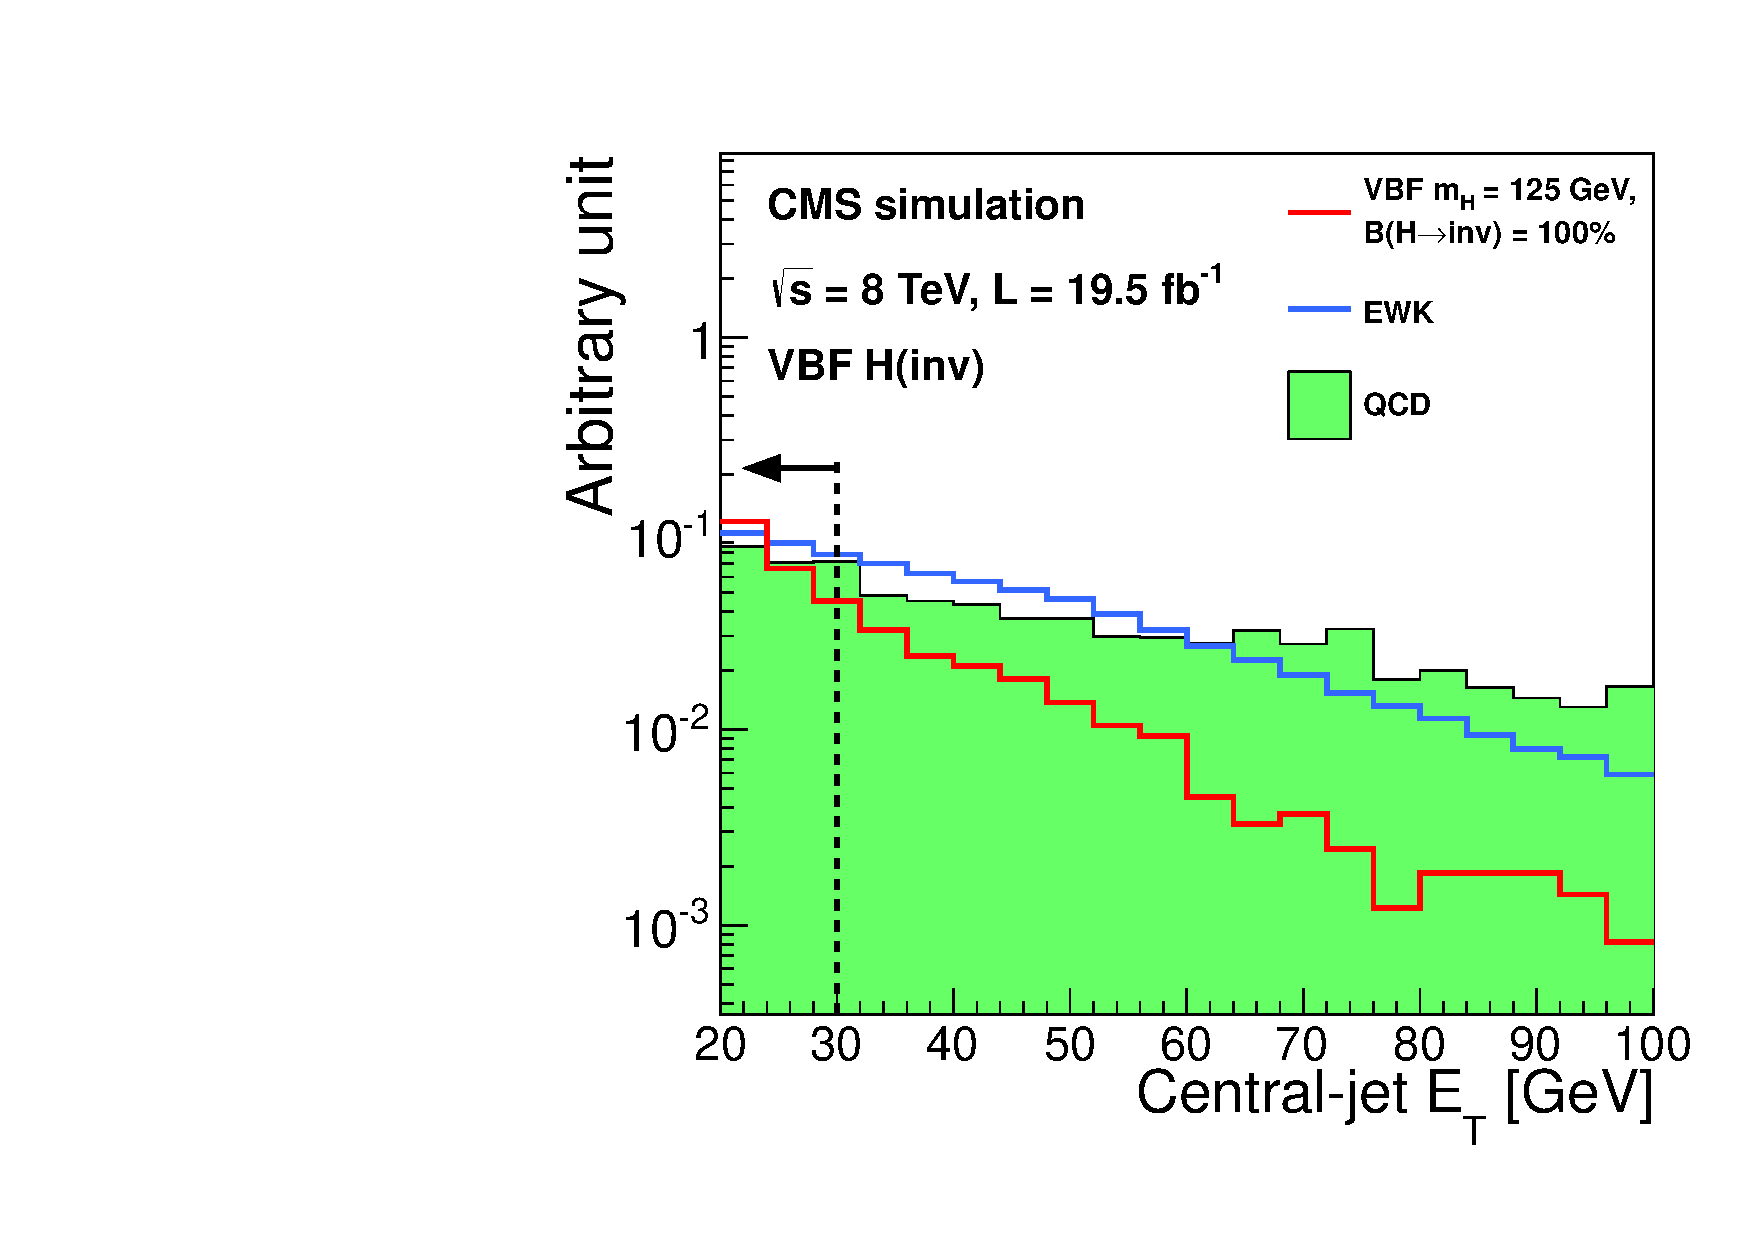
\includegraphics[width=.65\largefigwidth]{plots/prompt/VBF-CJV-pT.pdf}}
  \caption{Distributions of (a) \Mjj, (b) \detajj, (c) \dphijj and (d) leading central jet \pt in background and signal MC events. The events shown are required to have two jets in opposite forward/backward halves of the detector with \pt$>50$ \GeV, $\Mjj>150$ \GeV and \METnoMU$>130$ \GeV. EWK refers to the V+jets and minor backgrounds described in \SectionRef{sec:promptbkg} and QCD refers to the QCD multijet background. The dashed lines indicate the offline selection criteria applied to these variables, which are motivated in the text ~\cite{Chatrchyan:2014tja}.}
  \label{fig:promptcontrolplots}
\end{figure}


\section{Background estimation}
\label{sec:promptbkg}
As discussed in \SectionRef{sec:promptsel} there are several background processes which are capable of producing VBF-like jets in association with \MET. The event selection removes most of these events, however a significant number still remain and it is important to estimate this number precisely. Data-driven methods, with data ``control regions'' which are similar to the signal region, are used to estimate the most significant backgrounds. This data-driven approach is particularly important as the very stringent kinematic requirements placed on the tag jets lead to large uncertainties on estimates taken from \ac{MC} alone. The particular method used to estimate each of the backgrounds will be described in this section. As described in the declaration, I performed a cross-check of the $\PW+$jets background estimation. The tables of the results of and inputs to the $\PW+$jets background estimation in this section are taken from this cross-check. Therefore, whilst the agreement with the published results is good, exact agreement is not expected.

\subsection{\PW$\rightarrow e\nu$ + jets}
\label{sec:promptwenu}
The $\PW+$jets background where the $\PW$ boson decays to an electron and an electron neutrino, $\PW\rightarrow e\nu$, is estimated using single electron events. All aspects of the event selection are the same as those used in the signal region, except for the electron veto, which is replaced with the requirement that there is exactly one tight electron in the event and no other veto electrons. These requirements give a single electron control region composed of events with jets that have the same kinematics as those in the signal region, but which is dominated by $\PW\rightarrow e\nu$ events.

The number of $\PW\rightarrow e\nu$ events in the signal region is then estimated by using the ratio between the expected number of events in the signal and control regions from \ac{MC} to extrapolate from the number of events seen in data in the single electron control region using the following formula:
\begin{equation}
  \label{eq:wdatabkg}
  N^{S}_{Exp}=\left(N^{C}_{Data}-N^{C}_{Bkg}\right)\cdot\frac{N^{S}_{MC}}{N^{C}_{MC}},
\end{equation}
where $N^{S}_{Exp}$ is the number of expected events in the signal region from this background process, $N^{C}_{Data}$ is the number of events seen in the control region in data, $N^{C}_{Bkg}$ is the number of events from other backgrounds in the control region estimated using \ac{MC}, which is expected to be small, and $N^{S}_{MC}$ and $N^{C}_{MC}$ are the numbers of events predicted by \ac{MC} to be in the signal and control regions respectively. The fact that estimations from \ac{MC} are only used in ratios, or where they are expected to be small, significantly reduces the dependence of the final background estimation on the overall rate of the process predicted by \ac{MC} and instead allows the observed rate in data to be used. It is important that the shape of the variables which differ between the control and signal regions are well modelled by the \ac{MC}. The modelling of the shape of two key variables, the \METnoMU and the electron \pt, are shown in \FigureRef{fig:promptwenu}. It can be seen that whilst the overall rate is significantly different between data and \ac{MC}, the shape of the distribution is modelled well. Furthermore, as a closure test $N^{S}_{MC}$ was replaced with the number of \ac{MC} events expected in the control regions used for other background processes and good agreement was seen. The inputs to, and results of, the background estimation are shown in \TableRef{tab:promptwenu}.

%tables from AN-13-205
\begin{table}
  \caption{The inputs to, and results of, the cross-check performed by the author of the $\PW\rightarrow e\nu$ background estimation. $N_{\PW\rightarrow e\nu}$ is, for the signal region the number of events expected from $\PW\rightarrow e\nu$ backgrounds, and for the control region the number of events remaining in the region after the subtraction of other backgrounds.}
  \label{tab:promptwenu}
  \begin{tabular}{lcc}
    \hline
    \hline
    & Signal region & Control region \\
    \hline
    \hline
    $N_{Data}$ & N/A & 64\\
    $N_{Bkg}$ & N/A & $7.42\pm2.78$(\ac{MC} stat.) \\
    $N_{MC}$& $105\pm10$(\ac{MC} stat.) & $86.6\pm 7.1$(\ac{MC} stat.) \\
    \hline
    $\frac{N^{data}-N^{bkg}}{N^{C}_{MC}}$ & \multicolumn{2}{c|}{0.65$\pm$0.09\stat$\pm$0.06(MC stat)} \\
    \hline
    $N_{\PW\rightarrow e\nu}$& \textcolor{red}{$68.7\pm 10.3\stat\pm 8.8$(MC stat.)} & $56.6\pm 8.5\stat$ \\
    \hline
    \hline
  \end{tabular}
\end{table}

%plot from AN-12-403
\begin{figure}
  \subfloat[]{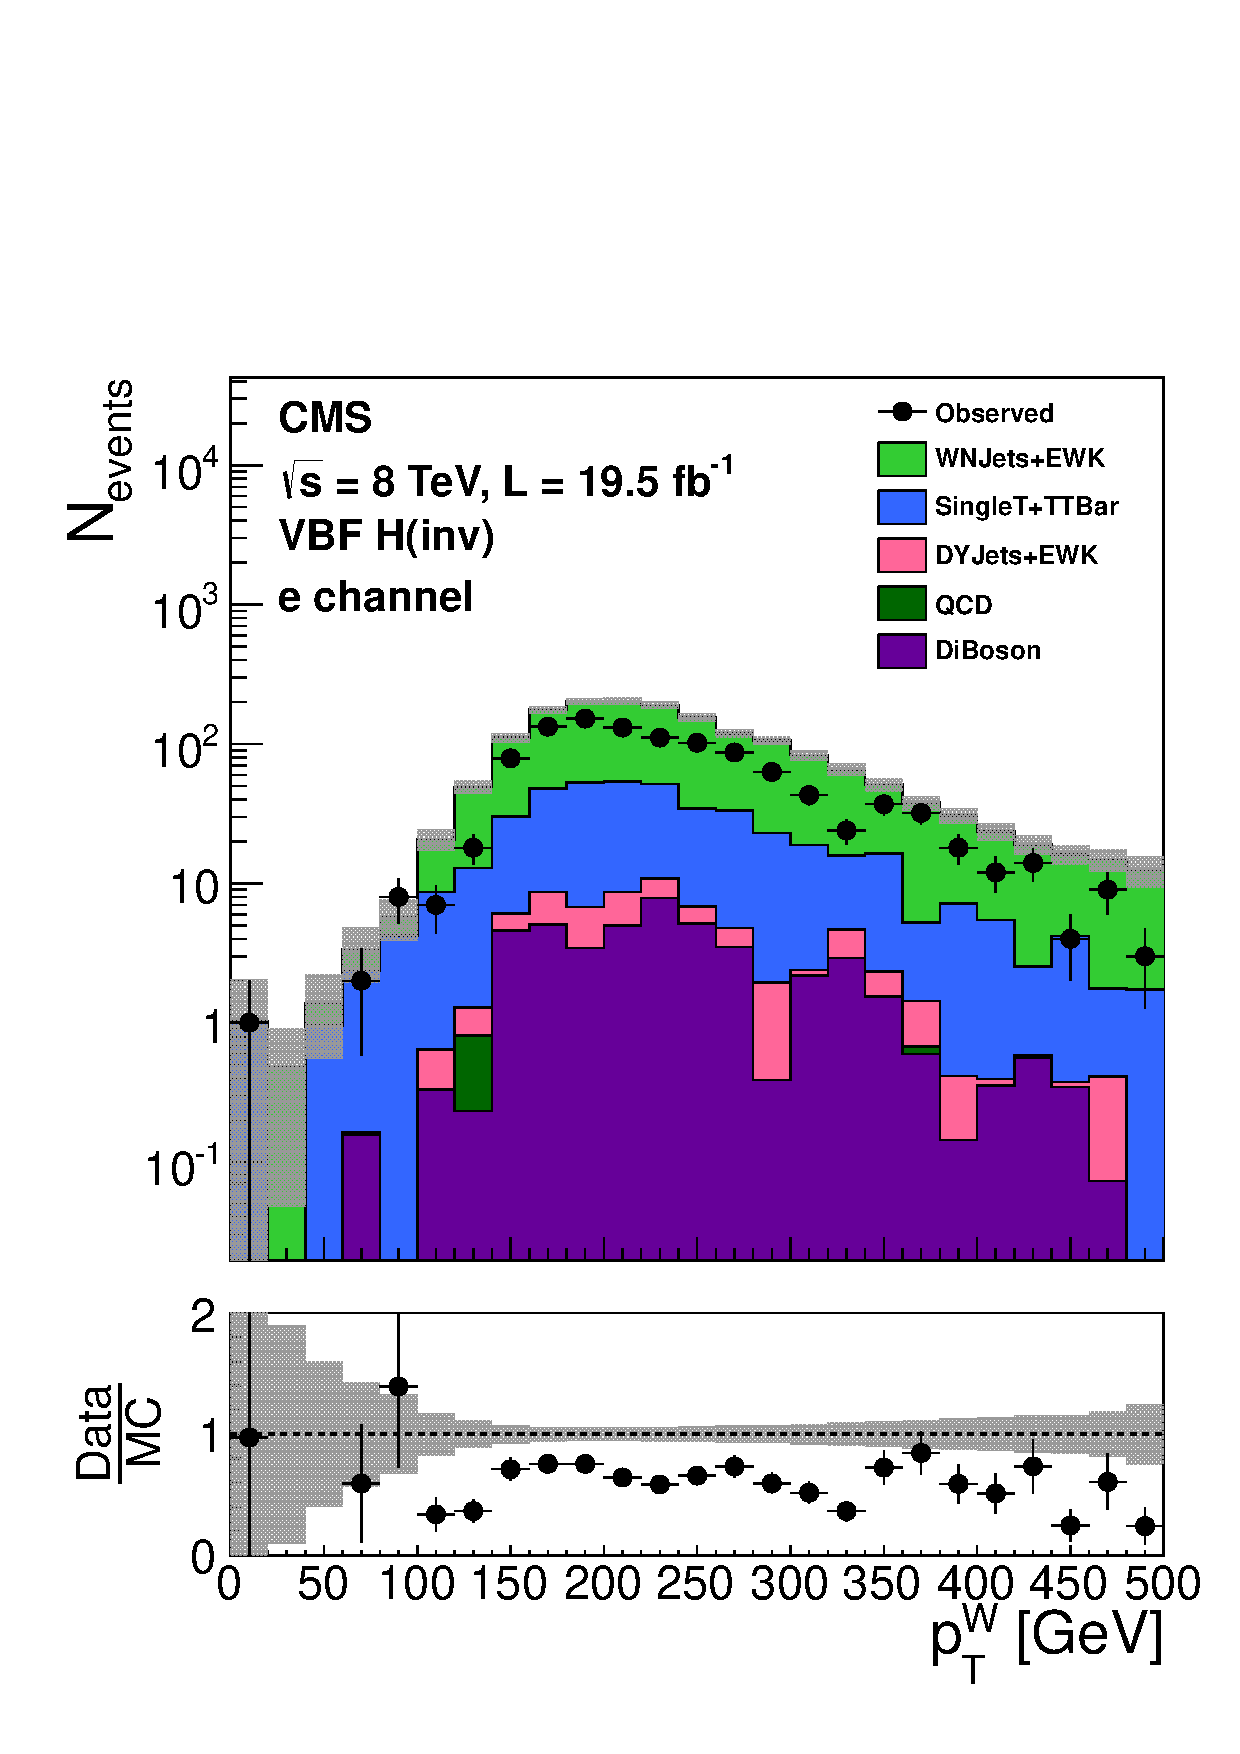
\includegraphics[width=.65\largefigwidth]{plots/prompt/AN-12-403-figs/hWEl_WpT.pdf}}
  \subfloat[]{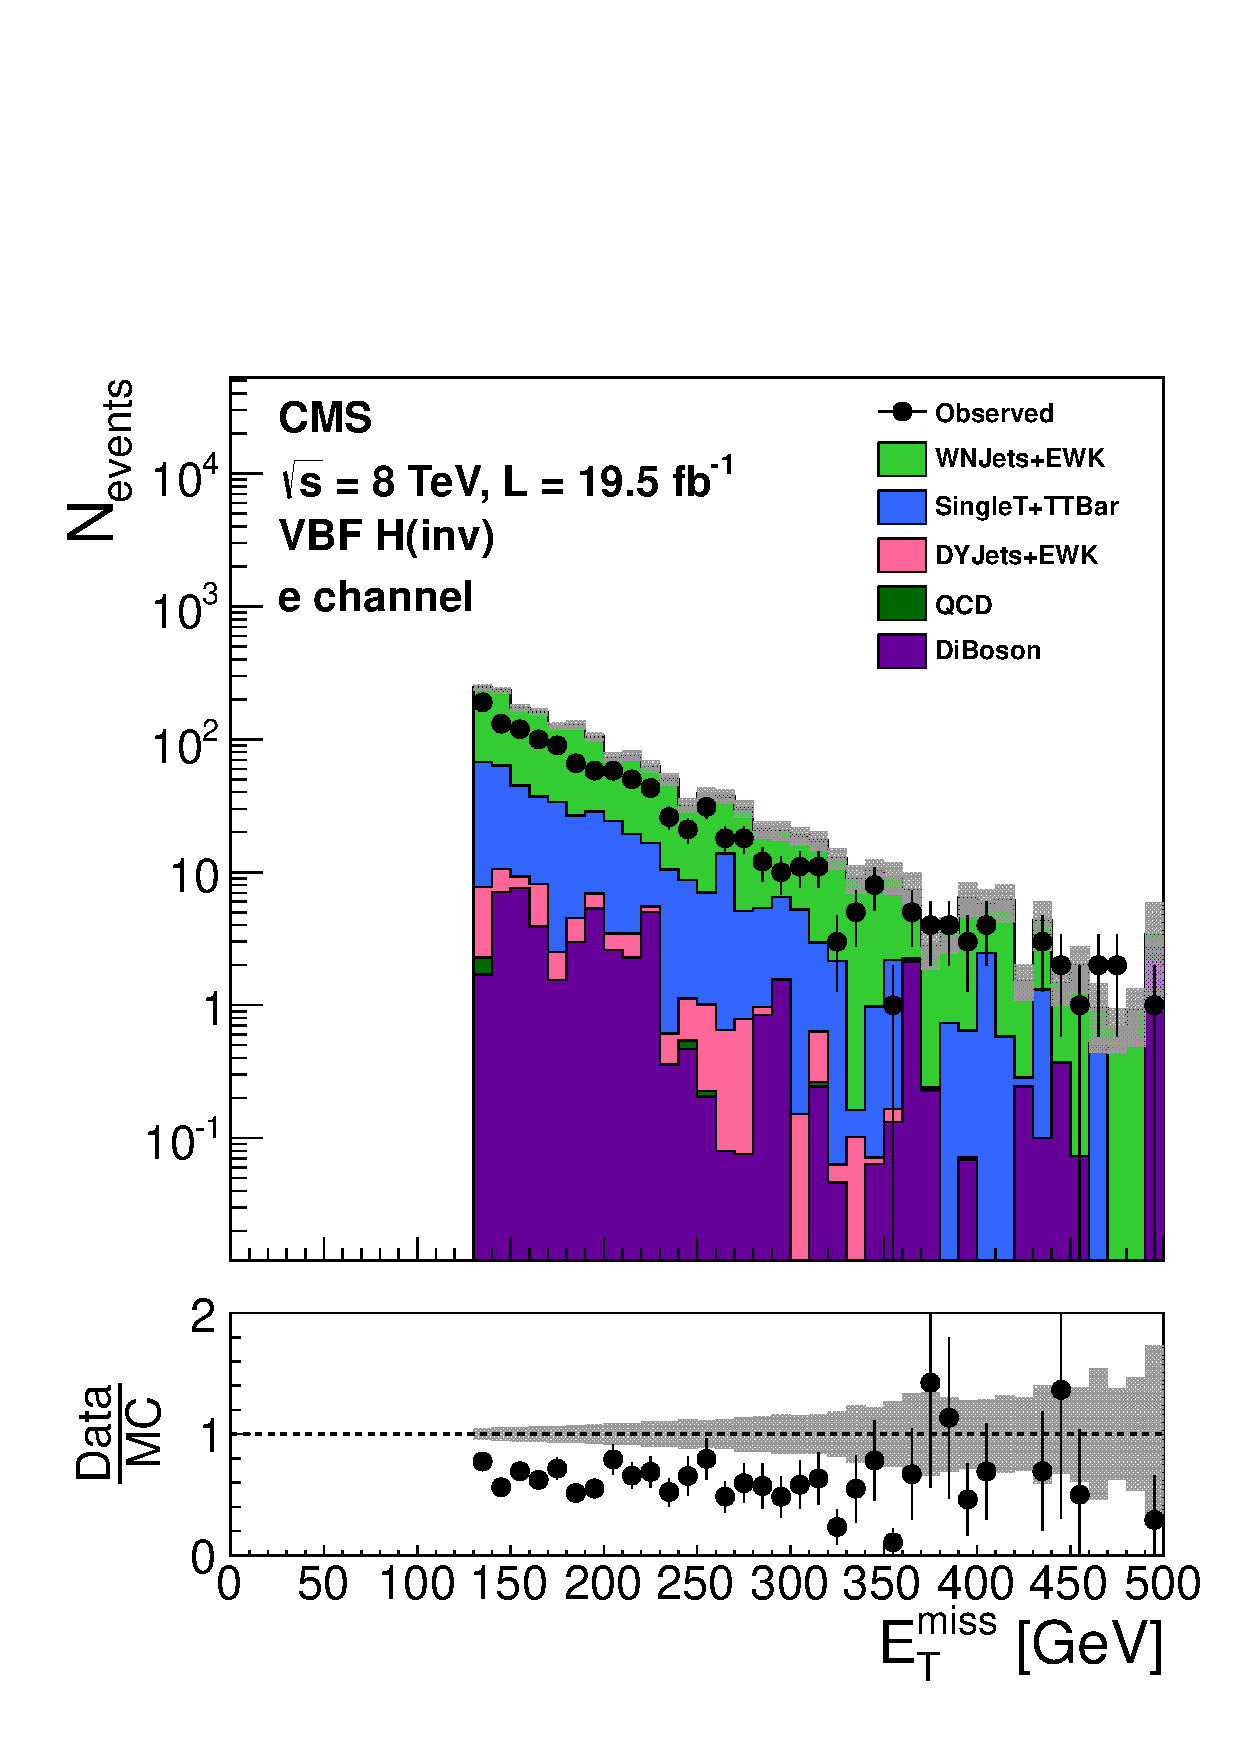
\includegraphics[width=.65\largefigwidth]{plots/prompt/AN-12-403-figs/hWEl_MET.pdf}}
  \caption{Distributions of the visible $\PW$ boson \pt (i.e. the electron \pt) (a) and \METnoMU (b) in the single electron control region. WNJets+EWK indicates the W+jets contribution to this region, SingleT+TTBar indicates the contribution from top quark related processes, DYJets+EWK indicates the Z+jets contribution, QCD indicates the QCD multijet contribution and DiBoson indicates the two vector boson contribution. All of these contributions are estimated from MC. The hatched region illustrates the systematic uncertainty~\cite{ARTICLE:CMSAN-12-403}. Whilst the overall rate of data and MC is very different, the shape can be seen to agree well.}
  \label{fig:promptwenu}
\end{figure}

\subsection{\PW$\rightarrow \mu\nu$ + jets}
\label{sec:promptwmunu}
The method used to estimate the background from $\PW$+jets where the $\PW$ boson decays to a muon and a muon neutrino, $\PW\rightarrow\mu\nu$, is very similar to that used for $\PW\rightarrow e\nu$. A single muon control region is used which replaces the muon veto of the signal region with a requirement that there is exactly one tight muon and no other veto muons. All other signal region cuts remain unchanged. Equation \ref{eq:wdatabkg} is then used, with the control region now being the single muon control region, to estimate the number of events from $W\rightarrow\mu\nu$ expected in the signal region. The inputs to, and results of, the background estimation are shown in \TableRef{tab:promptwmunu}, and distributions of the muon \pt and the \METnoMU in the single muon control region are shown in \FigureRef{fig:promptwmunu}.

%tables from AN-13-205
\begin{table}
  \caption{The inputs to, and results of, the $\PW\rightarrow \mu\nu$ background estimation. $N_{\PW\rightarrow \mu\nu}$ is, for the signal region the number of events expected from $\PW\rightarrow \mu\nu$ backgrounds, and for the control region the number of events remaining in the region after the subtraction of other backgrounds.}
  \label{tab:promptwmunu}
  \begin{tabular}{lcc}
    \hline
    \hline
    & Signal region & Control region \\
    \hline
    \hline
    $N_{Data}$ & N/A & 216\\
    $N_{Bkg}$ & N/A & $30.1\pm 4.5$(\ac{MC} stat.) \\
    $N_{MC}$& $108\pm 10$(\ac{MC} stat.) & $306\pm 15$(\ac{MC} stat.) \\
    \hline
    $\frac{N^{data}-N^{bkg}}{N^{C}_{MC}}$ & \multicolumn{2}{c|}{$0.61\pm$0.05\stat$\pm$0.03(MC stat)} \\
    \hline
    $N_{\PW\rightarrow \mu\nu}$& \textcolor{red}{$65.8\pm 5.4\stat\pm 6.7$(MC stat.)} & $186\pm 15\stat$ \\
    \hline
    \hline
  \end{tabular}
\end{table}

%plot from AN-12-403
\begin{figure}
  \subfloat[]{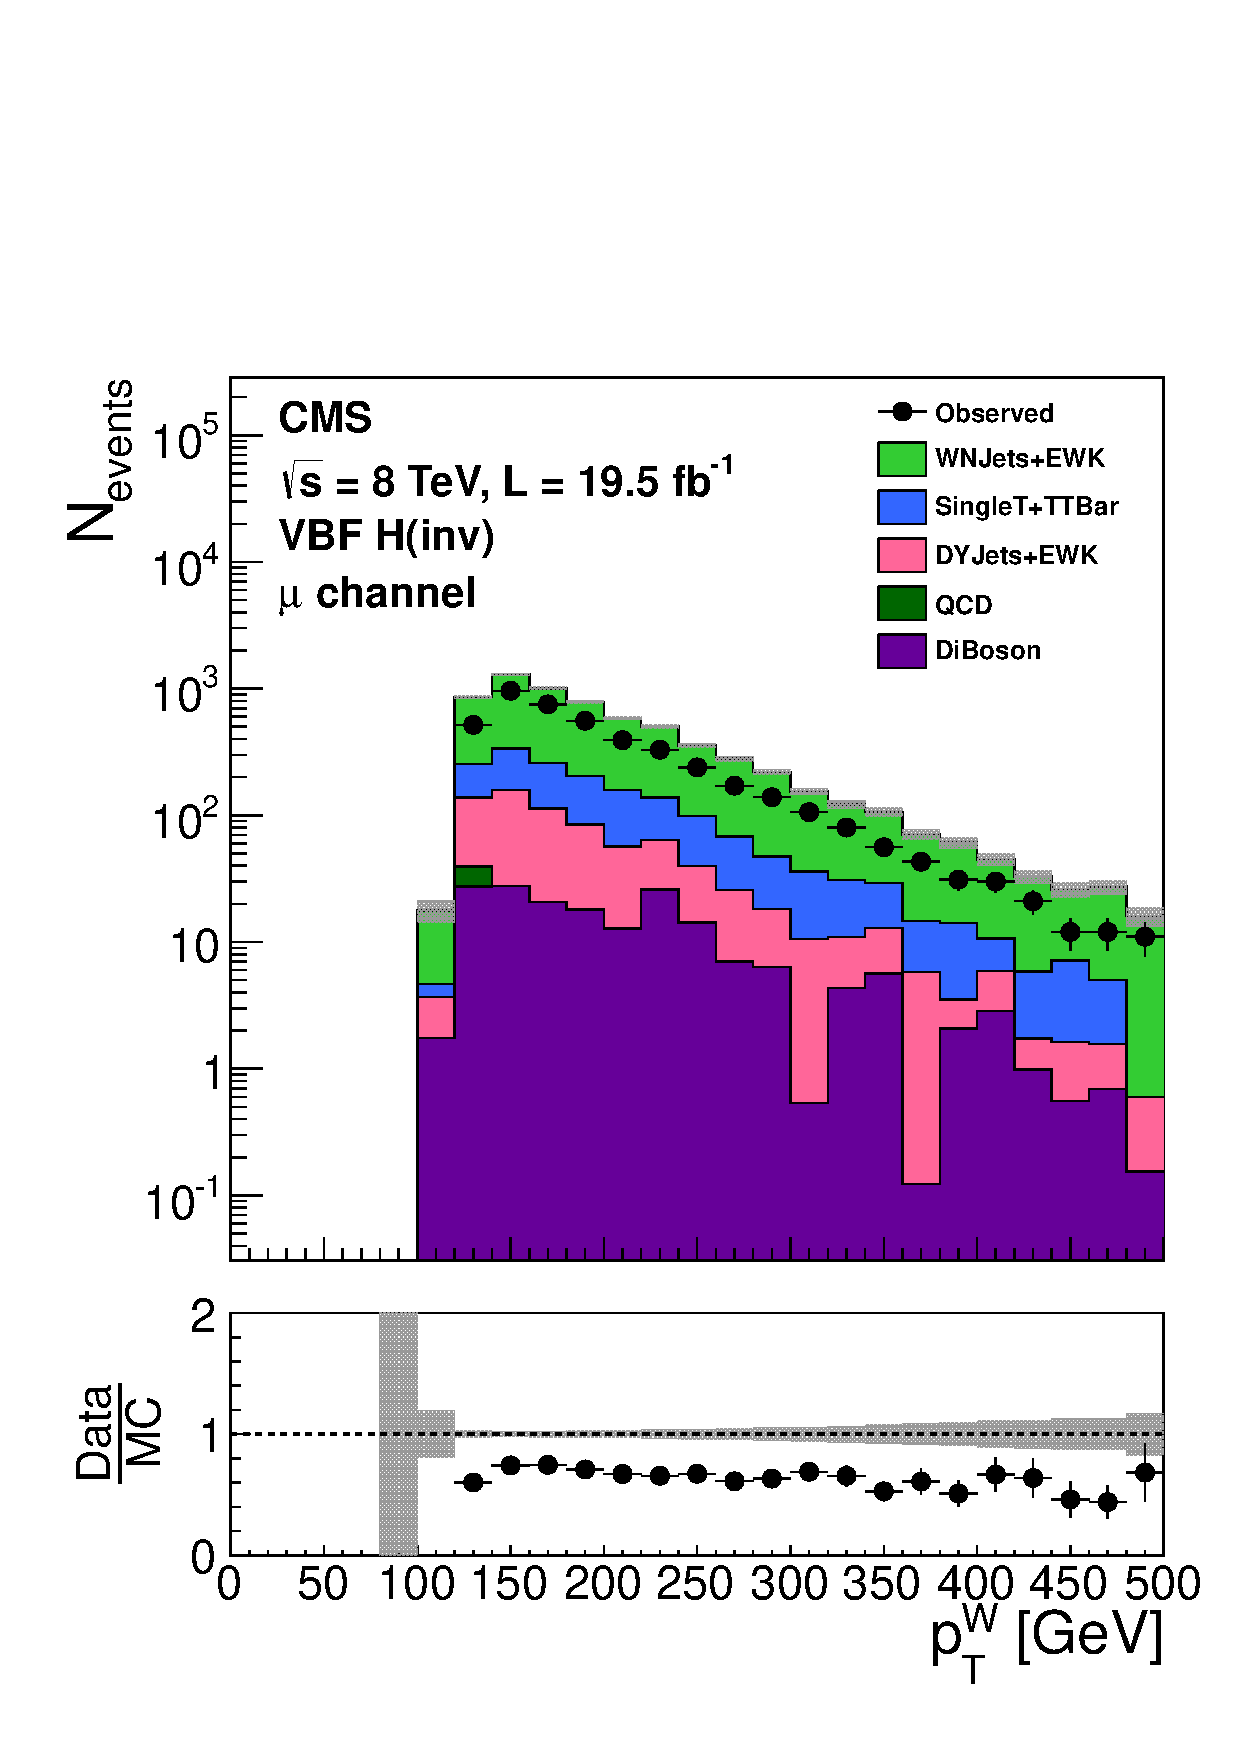
\includegraphics[width=.65\largefigwidth]{plots/prompt/AN-12-403-figs/hWMu_WpT.pdf}}
  \subfloat[]{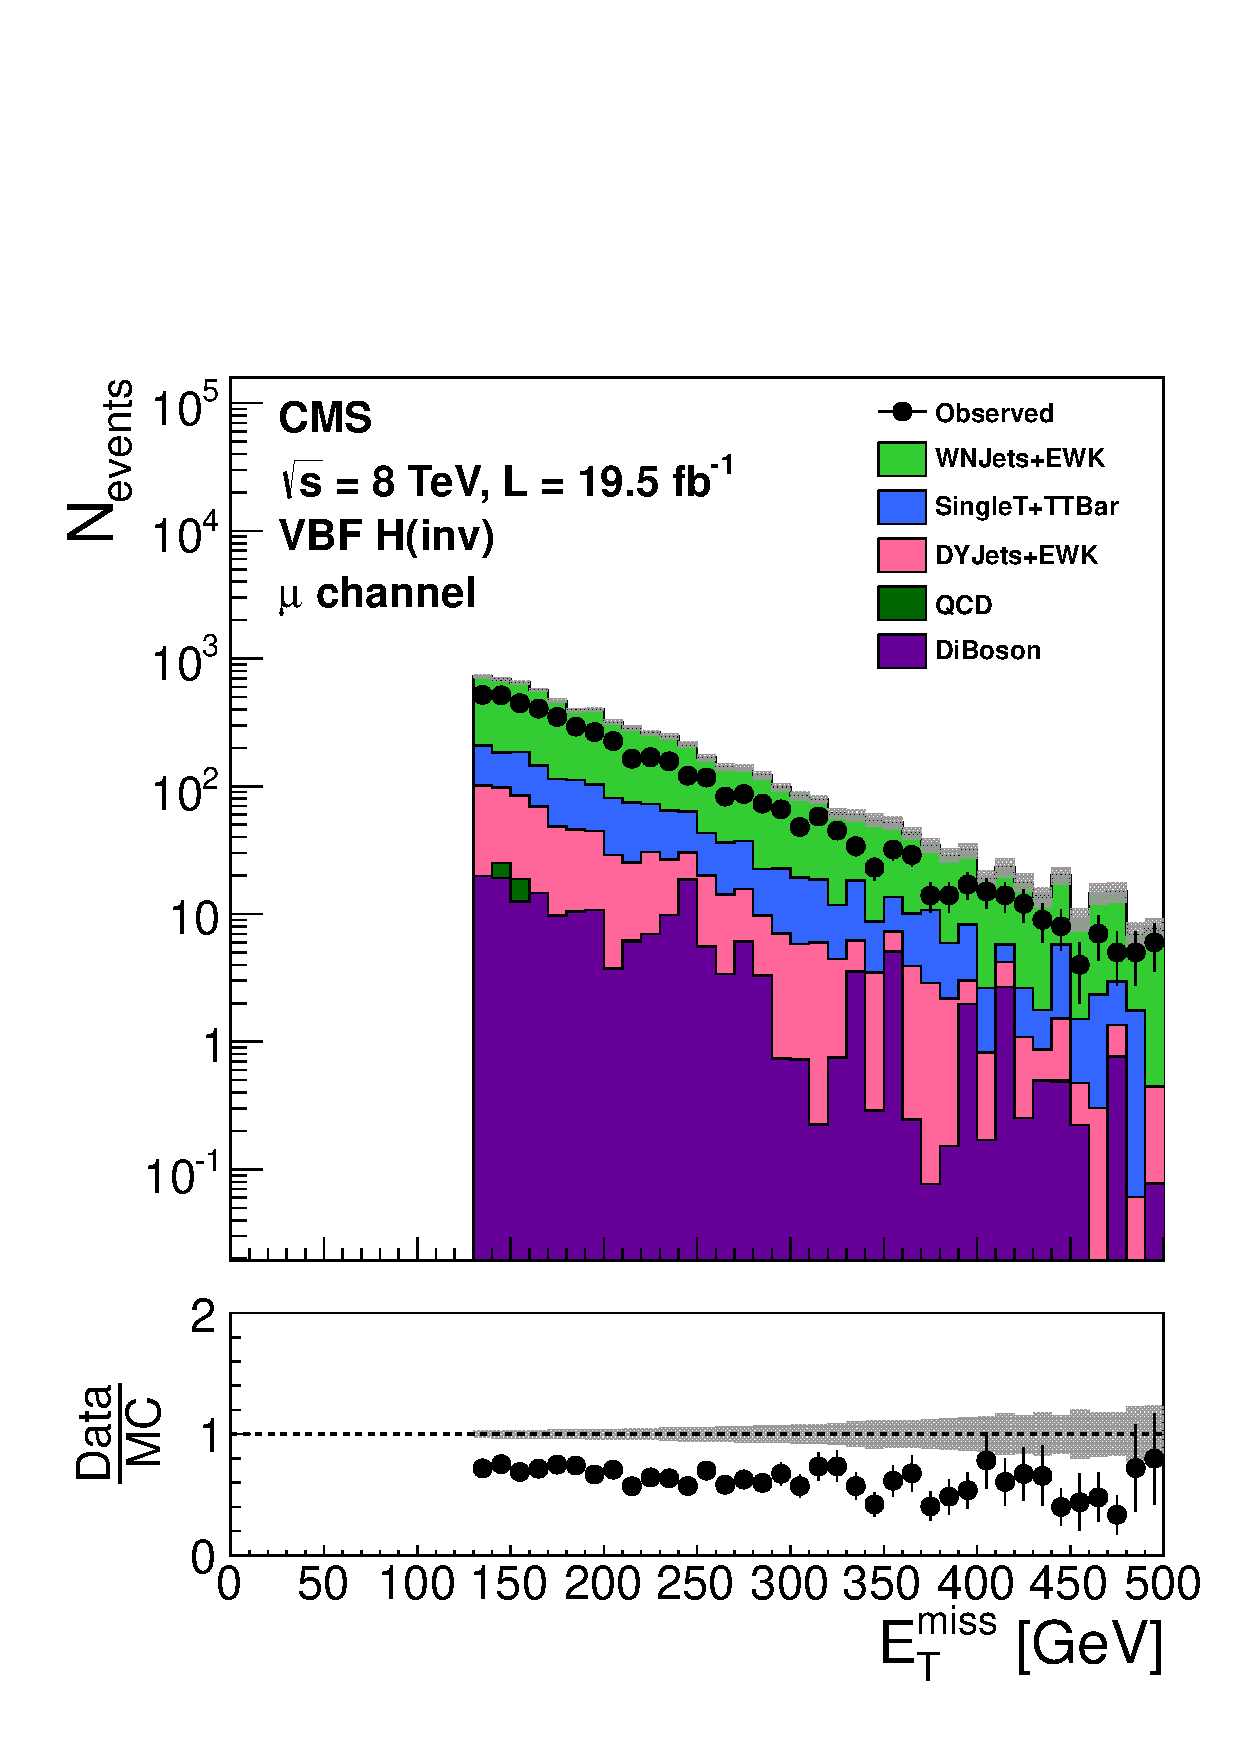
\includegraphics[width=.65\largefigwidth]{plots/prompt/AN-12-403-figs/hWMu_MET.pdf}}
  \caption{Distributions of the visible $\PW$ boson \pt (i.e. the muon \pt) (a) and \METnoMU (b) in the single muon control region. WNJets+EWK indicates the W+jets contribution to this region, SingleT+TTBar indicates the contribution from top quark related processes, DYJets+EWK indicates the Z+jets contribution, QCD indicates the QCD multijet contribution and DiBoson indicates the two vector boson contribution. All of these contributions are estimated from MC. The hatched region illustrates the systematic uncertainty~\cite{ARTICLE:CMSAN-12-403}. Whilst the overall rate of data and MC is very different, the shape can be seen to agree well.}
  \label{fig:promptwmunu}
\end{figure}

\subsection{\PW$\rightarrow \tau\nu$ + jets}
\label{sec:promptwtaunu}
The background from $\PW$+jets where the $\PW$ boson decays to a tau and a tau neutrino, $\PW\rightarrow\tau\nu$, is estimated using a single tau control region data-driven method. However, in this case the control region used has more differences from the signal region than those used above. The reason for these increased differences is that the reconstruction efficiency for tau leptons is significantly lower than that for electrons or muons, and they are also more likely to be misreconstructed as jets, causing the event to be vetoed by the \ac{CJV}. There are therefore only $3.76\pm 1.27\stat$ $\PW\rightarrow\tau\nu$ events with identified taus with \pt$>20$ \GeV expected in the signal region from \ac{MC}.

To increase the number of events in the single tau control region, the \ac{CJV} has been removed. The resulting control region has $29.2\pm 3.61\stat$ $\PW+$jets events expected and thus a much lower statistical uncertainty. As there is no veto of tau leptons in the signal region the tau control region and the signal region are not mutually exclusive. However, as stated above the number of events in the signal region with identified taus is expected to be small, so the overlap is considered negligible.

%cross-check of tau discriminant https://indico.cern.ch/event/259915/session/1/contribution/2/attachments/458506/635408/tauid090713.pdf
In addition to the tau identification algorithm described in \SectionRef{sec:taus}, alternative algorithms were studied to check for better performance in terms of identification efficiency and fake rate. Specifically, an alternative isolation algorithm was investigated which used a \ac{MVA} approach to estimate the isolation sum, as well as different working points for the anti-electron and anti-muon discriminators~\cite{CMS-PAS-TAU-11-001}. The tau identification efficiency was found to be higher for both the alternative isolation algorithm and different working points for the anti-lepton discriminators, being twice as large if both were used compared to the standard tau identification. However, the rate of $\PW\rightarrow e\nu$ events being identified as $\PW\rightarrow\tau\nu$ was also significantly increased, going from 2\% for the standard identification to 15\% when the alternative isolation and anti-lepton discriminators were used. It was therefore decided to use the tau identification described in \SectionRef{sec:taus}.

The final estimation of the background from $W\rightarrow\tau\nu$ is carried out using \EquationRef{eq:wdatabkg}, with the single tau control region with no \ac{CJV} being used as the control region. The inputs to, and results of, the background estimation are shown in \TableRef{tab:promptwtaunu}. Distributions of the tau \pt and \dphijj in the single tau control region are shown in \FigureRef{fig:promptwtaunu}; it can be seen that the shape of the two distributions in data and \ac{MC} agree well with the exception of the high \dphijj region which is not part of either the signal or tau control regions.

%tables from AN-13-205
\begin{table}
  \caption{The inputs to, and results of, the $\PW\rightarrow \tau\nu$ background estimation. $N_{\PW\rightarrow \tau\nu}$ is, for the signal region the number of events expected from $\PW\rightarrow \tau\nu$ backgrounds, and in the control region the number of events remaining in the region after the subtraction of other backgrounds.}
  \label{tab:promptwtaunu}
  \begin{tabular}{lcc}
    \hline
    \hline
    & Signal region & Control region \\
    \hline
    \hline
    $N_{Data}$ & N/A & 32\\
    $N_{Bkg}$ & N/A & $14.7\pm 3.4$(\ac{MC} stat.) \\
    $N_{MC}$& $95.6\pm 8.5$(\ac{MC} stat.) & $29.2\pm 3.6$(\ac{MC} stat.) \\
    \hline
    $\frac{N^{data}-N^{bkg}}{N^{C}_{MC}}$ & \multicolumn{2}{c|}{$0.59\pm$0.19\stat$\pm$0.10(MC stat)} \\
    \hline
    $N_{\PW\rightarrow \tau\nu}$& \textcolor{red}{$56.5\pm 21.5\stat\pm 8.6$(MC stat.)} & $17.3\pm 3.9 \stat$ \\
    \hline
    \hline
  \end{tabular}
\end{table}

%plot from AN-12-403
\begin{figure}
  \subfloat[]{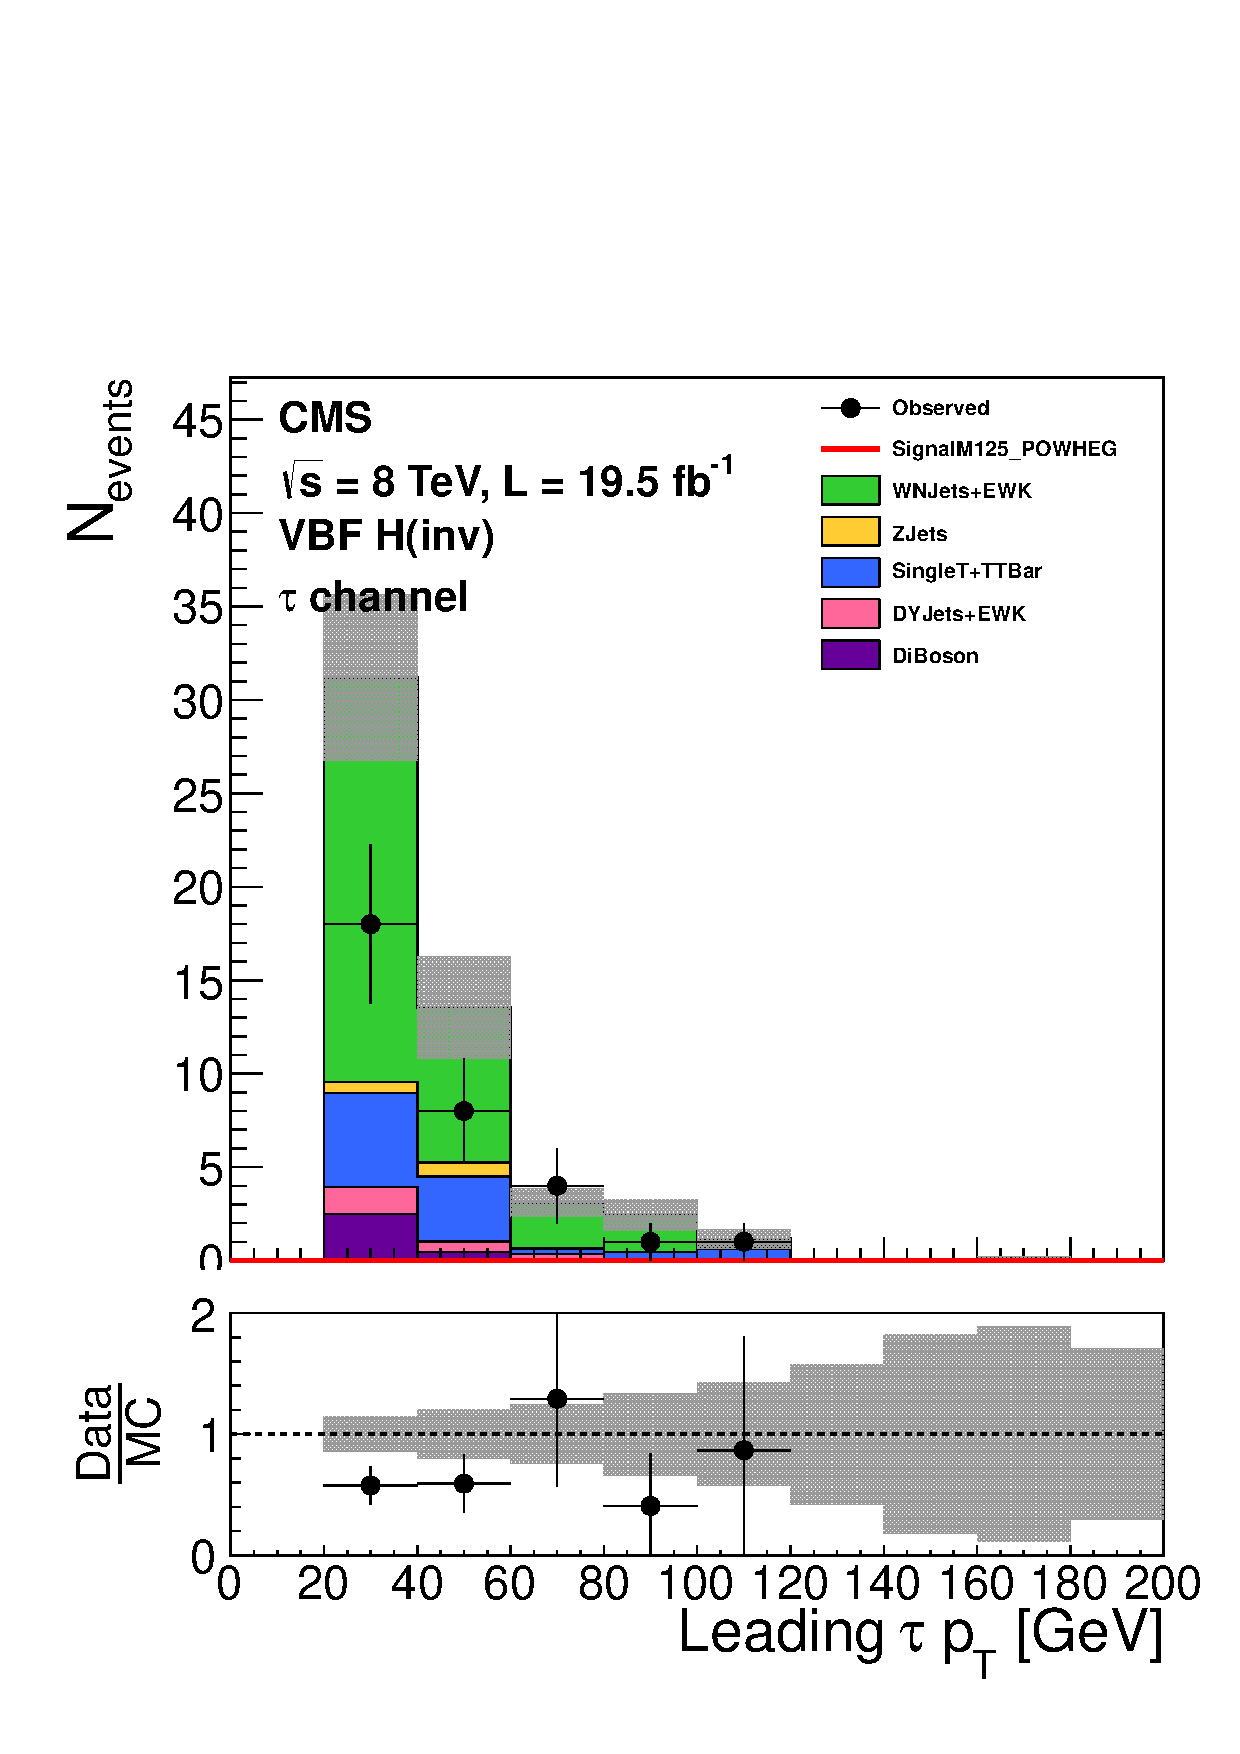
\includegraphics[width=.65\largefigwidth]{plots/prompt/AN-12-403-figs/hWTau_tau1Pt.pdf}}
  \subfloat[]{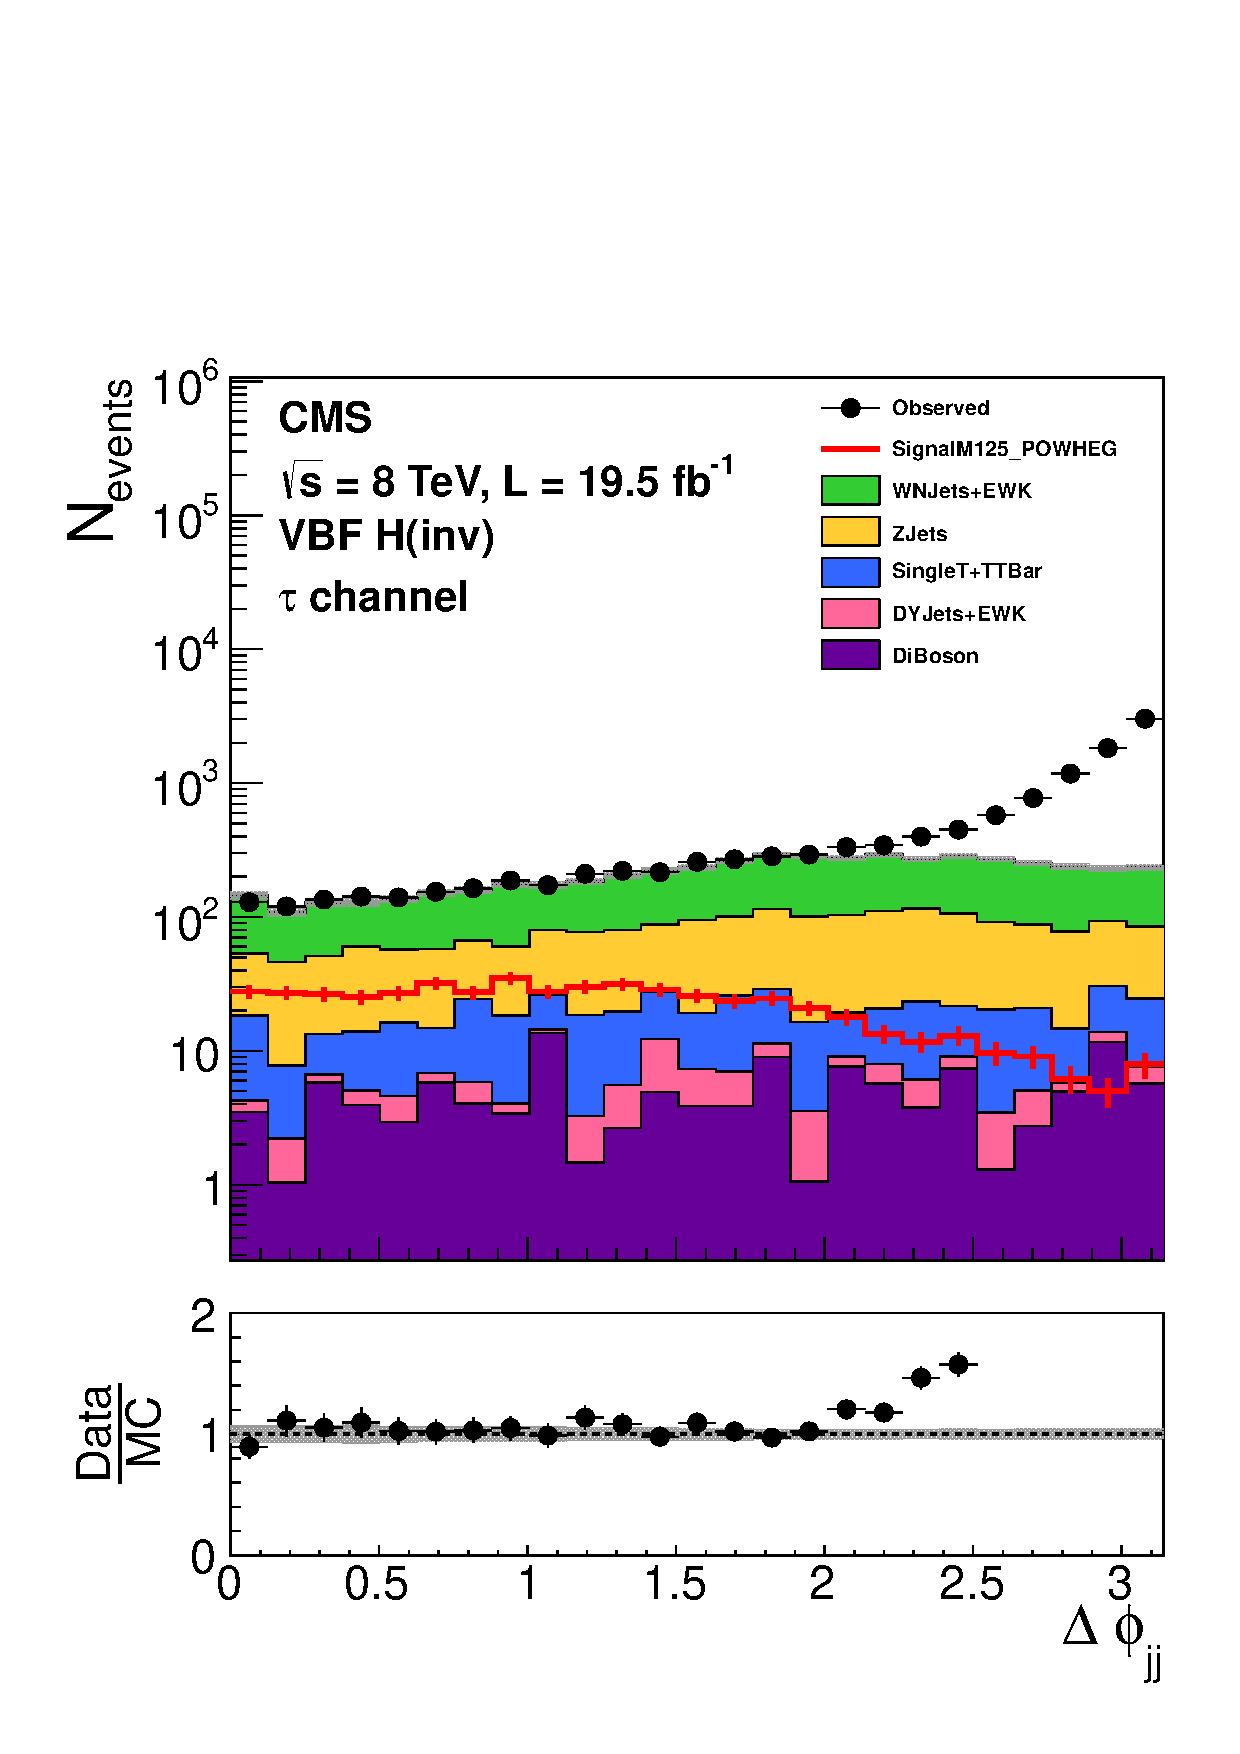
\includegraphics[width=.65\largefigwidth]{plots/prompt/AN-12-403-figs/hWTau_dPhiJJ.pdf}}
  \caption{Distributions of the the tau \pt (a) and \dphijj (b) in the single tau control region. WNJets+EWK indicates the W+jets contribution to this region, ZJets indicates the contribution from Z+jets, SingleT+TTBar indicates the contribution from top quark related processes, QCD indicates the QCD multijet contribution and DiBoson indicates the two vector boson contribution. All of these contributions are estimated from MC. The hatched region illustrates the systematic uncertainty~\cite{ARTICLE:CMSAN-12-403}.}
  \label{fig:promptwtaunu}
\end{figure}

\subsection{\PZ$\rightarrow \nu\nu$ + jets}
\label{sec:promptznunu}
The background from $\PZ+$jets where the \PZ decays to neutrinos, \Znunu, is different from the $\PW+$jets backgrounds described above, in that nothing is required to be misidentified in order for these events to contribute to the signal region. The method used to estimate the \Znunu background therefore differs slightly from that used above. The method uses a dimuon control region which is populated by events from the process \Zmumu. As this process can be mediated by a photon, the kinematics of the jets in \Zmumu events can be different to those from \Znunu. The dimuon control region that is defined therefore has a requirement that the invariant mass of the dimuons be between 60 and 120 \GeV. The control region is otherwise identical to the signal region, except that the muon veto is replaced with a requirement that there are exactly two tight muons and no other veto muons.

As well as the possibility of different kinematics, \Zmumu and $\PZ\rightarrow\nu\nu$ also have different cross-sections. The formula used to estimate the $\PZ\rightarrow\nu\nu$ background takes this into account as follows:
\begin{equation}
  \label{eq:zdatabkg}
  N^{S}_{Exp}=\left(N^{C}_{Data}-N^{C}_{Bkg}\right)\cdot\frac{\sigma\left(\PZ\rightarrow\nu\nu\right)}{\sigma\left(\PZ/\gamma^{*}\rightarrow\mu\mu\right)}\cdot\frac{\epsilon^{S}_{\mbox{VBF}}}{\epsilon^{C}_{\mbox{VBF}}},
\end{equation}
where $\sigma\left(\PZ\rightarrow\nu\nu\right)$ is the cross-section for \Znunu and $\sigma\left(\PZ/\gamma^{*}\rightarrow\mu\mu\right)$ is the cross-section for \Zmumu. $\epsilon^{S}_{\mbox{VBF}}$ and $\epsilon^{C}_{\mbox{VBF}}$ are the efficiencies for $Z\rightarrow\nu\nu$ events to pass the signal region selection and $Z/\gamma^{*}\rightarrow\mu\mu$ events to pass the control region selection respectively. As Z bosons can be created via either \ac{QCD} (those where the vertex where the \PZ boson is created is the only electroweak vertex) or electroweak processes (those where there are multiple electroweak vertices), which both have different cross-sections and efficiencies, $\epsilon^{S}_{\mbox{VBF}}$ and $\epsilon^{C}_{\mbox{VBF}}$, are a cross-section weighted average of the efficiency for both types of production, calculated as:
\begin{align}
  \label{eq:zdataeffs}
  \epsilon^{S}_{\mbox{VBF}}&=\frac{ \sigma\left(\PZ\rightarrow\nu\nu,EWK\right) \frac{N^{S}_{MC}\left(EWK\right)} {N_{gen}\left(\PZ \rm{mass},EWK\right)} + \sigma\left(\PZ\rightarrow\nu\nu,QCD\right) \frac{N^{S}_{MC}\left(QCD\right)} {N_{gen}\left(\PZ \rm{mass},QCD\right)} } {\sigma\left(\PZ\rightarrow\nu\nu,EWK\right) + \sigma\left(\PZ\rightarrow\nu\nu,QCD\right)},\\
  \label{eq:zdataeffc}
  \epsilon^{C}_{\mbox{VBF}}&=\frac{  \sigma\left(\PZ/\gamma^{*}\rightarrow\mu\mu,EWK\right) \frac{N^{C}_{MC}\left(EWK\right)} {N_{gen}\left(EWK\right)} + \sigma\left(\PZ/\gamma^{*}\rightarrow\mu\mu,QCD\right) \frac{N^{C}_{MC}\left(QCD\right)} {N_{gen}\left(QCD\right)}  }{\sigma\left(\PZ/\gamma^{*}\rightarrow\mu\mu,EWK\right)+\sigma\left(\PZ/\gamma^{*}\rightarrow\mu\mu,QCD\right)},
\end{align}
where $EWK$ and $QCD$ denote where cross-sections or numbers of events are for electroweak or \ac{QCD} production of a $\PZ$ boson. $N_{gen}$ is the number of events in the Z+jets \ac{MC} sample at generator-level. Due to the limited size of the available \Znunu \ac{MC} samples, the same \Zmumu samples used for the \ac{MC} estimate of the number of events in the control region are used to obtain an estimate from \ac{MC} of the number of events from the \Znunu process in the signal region. For this estimate the leptons in the \Zmumu samples are ignored, the production cross-section is scaled to the appropriate \Znunu value and it is required that there is a generator level dimuon in the event with invariant mass between 80 and 100 \GeV. The generated dimuon mass for this sample was required to be greater than 50 \GeV, so the cross-sections used in Equations~\ref{eq:zdatabkg}, \ref{eq:zdataeffs} and \ref{eq:zdataeffc} are also calculated with this constraint. For the control region $N_{gen}$ is calculated after requiring that the mass of the generator level dimuon is between 60 and 120 \GeV, denoted by the label ``$\PZ \rm{mass}$'' in Equations~\ref{eq:zdataeffs} and \ref{eq:zdataeffc}.


The inputs to Equations \ref{eq:zdataeffs} and \ref{eq:zdataeffc} are given in \TableRef{tab:promptznunueffs}. The cross-sections for electroweak $\PZ$ boson production were calculated at \ac{NLO} using \textsc{VBFNLO} which specialises in vector boson production. The cross-section for \ac{QCD} production of \Zmumu is calculated using \textsc{FEWZ} inclusively for all leptons and then divided by three to obtain the figure for muons only. This cross-section is then multiplied by the ratio between the cross-section for \Znunu and \Zmumu, which was calculated to be 5.651 at \ac{NLO} using \textsc{MCFM}, to obtain the \ac{QCD} production cross-section for \Znunu. The inputs to \EquationRef{eq:zdatabkg} are given in \TableRef{tab:promptznunu}, with the exception of the ratio between the total production cross-sections for \Znunu and \Zmumu which is taken to be the same 5.651 that it is found to be for \ac{QCD} production. This approximation is used because the electroweak contribution to the ratio is smaller than that from \ac{QCD} by more than a factor of one thousand and is therefore negligible. The distributions of \METnoMU and \Mjj for a \PZ control region with relaxed selection, to ensure sufficient numbers of events, are shown in \FigureRef{fig:promptznunu}, demonstrating that the \ac{MC} samples model the data distribution well.

%table from AN-12-403
\begin{table}
  \caption{The input variables for the calculation of $\epsilon^{S}_{\mbox{VBF}}$ and $\epsilon^{C}_{\mbox{VBF}}$ using Equations~\ref{eq:zdataeffs} and \ref{eq:zdataeffc} respectively.}
  \label{tab:promptznunueffs}
  \begin{tabular}{lc}
    \hline
    \hline
    Variable & Value \\
    \hline
    \hline
    $\sigma\left(\PZ\rightarrow\nu\nu,EWK\right)$ & 1.380~\pb\\
    $\sigma\left(\PZ\rightarrow\nu\nu,QCD\right)$ & 6600~\pb\\
    $\sigma\left(\PZ/\gamma^{*}\rightarrow\mu\mu,EWK\right)$ & 0.303~\pb\\
    $\sigma\left(\PZ/\gamma^{*}\rightarrow\mu\mu,QCD\right)$ & 1168~\pb\\
    \hline
    $\frac{N^{S}_{MC}(EWK)}{N_{gen}\left(\PZ\rm{mass},EWK\right)}$ & $\left(1.3\pm 0.1\right)\cdot 10^{-3}$ \\
    $\frac{N^{S}_{MC}(QCD)}{N_{gen}\left(\PZ\rm{mass},QCD\right)}$ & $\left(1.4\pm 0.2\right)\cdot 10^{-6}$\\
    $\frac{N^{C}_{MC}(EWK)}{N_{gen}\left(EWK\right)}$ & $\left(7.5\pm 0.3\right)\cdot 10^{-4}$\\
    $\frac{N^{C}_{MC}(QCD)}{N_{gen}\left(QCD\right)}$ & $\left(9.2\pm 1.2\right)\cdot 10^{-7}$\\
    \hline
    \hline
  \end{tabular}
\end{table}

\begin{table}
  \caption{The inputs to, and results of, the $\PZ\rightarrow \nu\nu$ background estimation using \EquationRef{eq:zdatabkg}. $\epsilon_{VBF}$ in the signal (control) region is calculated using Equation \ref{eq:zdataeffs} (\ref{eq:zdataeffc}).  $N_{\PZ\rightarrow \nu\nu}/N_{\PZ/\gamma^{*}\rightarrow\mu\mu}$ is in the signal region the number of events expected from $\PZ\rightarrow \nu\nu$ backgrounds, and for the control region the number of events remaining in the region after the subtraction of other backgrounds. The systematic uncertainties are calculated as described in \SectionRef{sec:promptsyst}.}
  \label{tab:promptznunu}
  \resizebox{1.0\linewidth}{!}{
    \begin{tabular}{lcc}
      \hline
      \hline
      & Signal region & Control region \\
      \hline
      \hline
      $N_{Data}$ & N/A & 12\\
      $N_{Bkg}$ & N/A & $0.3\pm 0.1$(\ac{MC} stat.) \\
      $\epsilon_{VBF}$& $(1.65 \pm 0.15\stat\pm 0.22\syst)\cdot 10^{-6}$ & $(1.11 \pm 0.12\stat\pm 0.12\syst)\cdot 10^{-6}$ \\
      \hline
      $N_{\PZ\rightarrow \nu\nu}/N_{\PZ\rightarrow/\gamma^{*}\rightarrow\mu\mu}$& \textcolor{red}{$99\pm 29\stat\pm 25\syst$} & $11.7\pm 0.1$(MC stat.) \\
      \hline
      \hline
    \end{tabular}
  }
\end{table}

%plot from HIG-13-030
\begin{figure}
  \subfloat[]{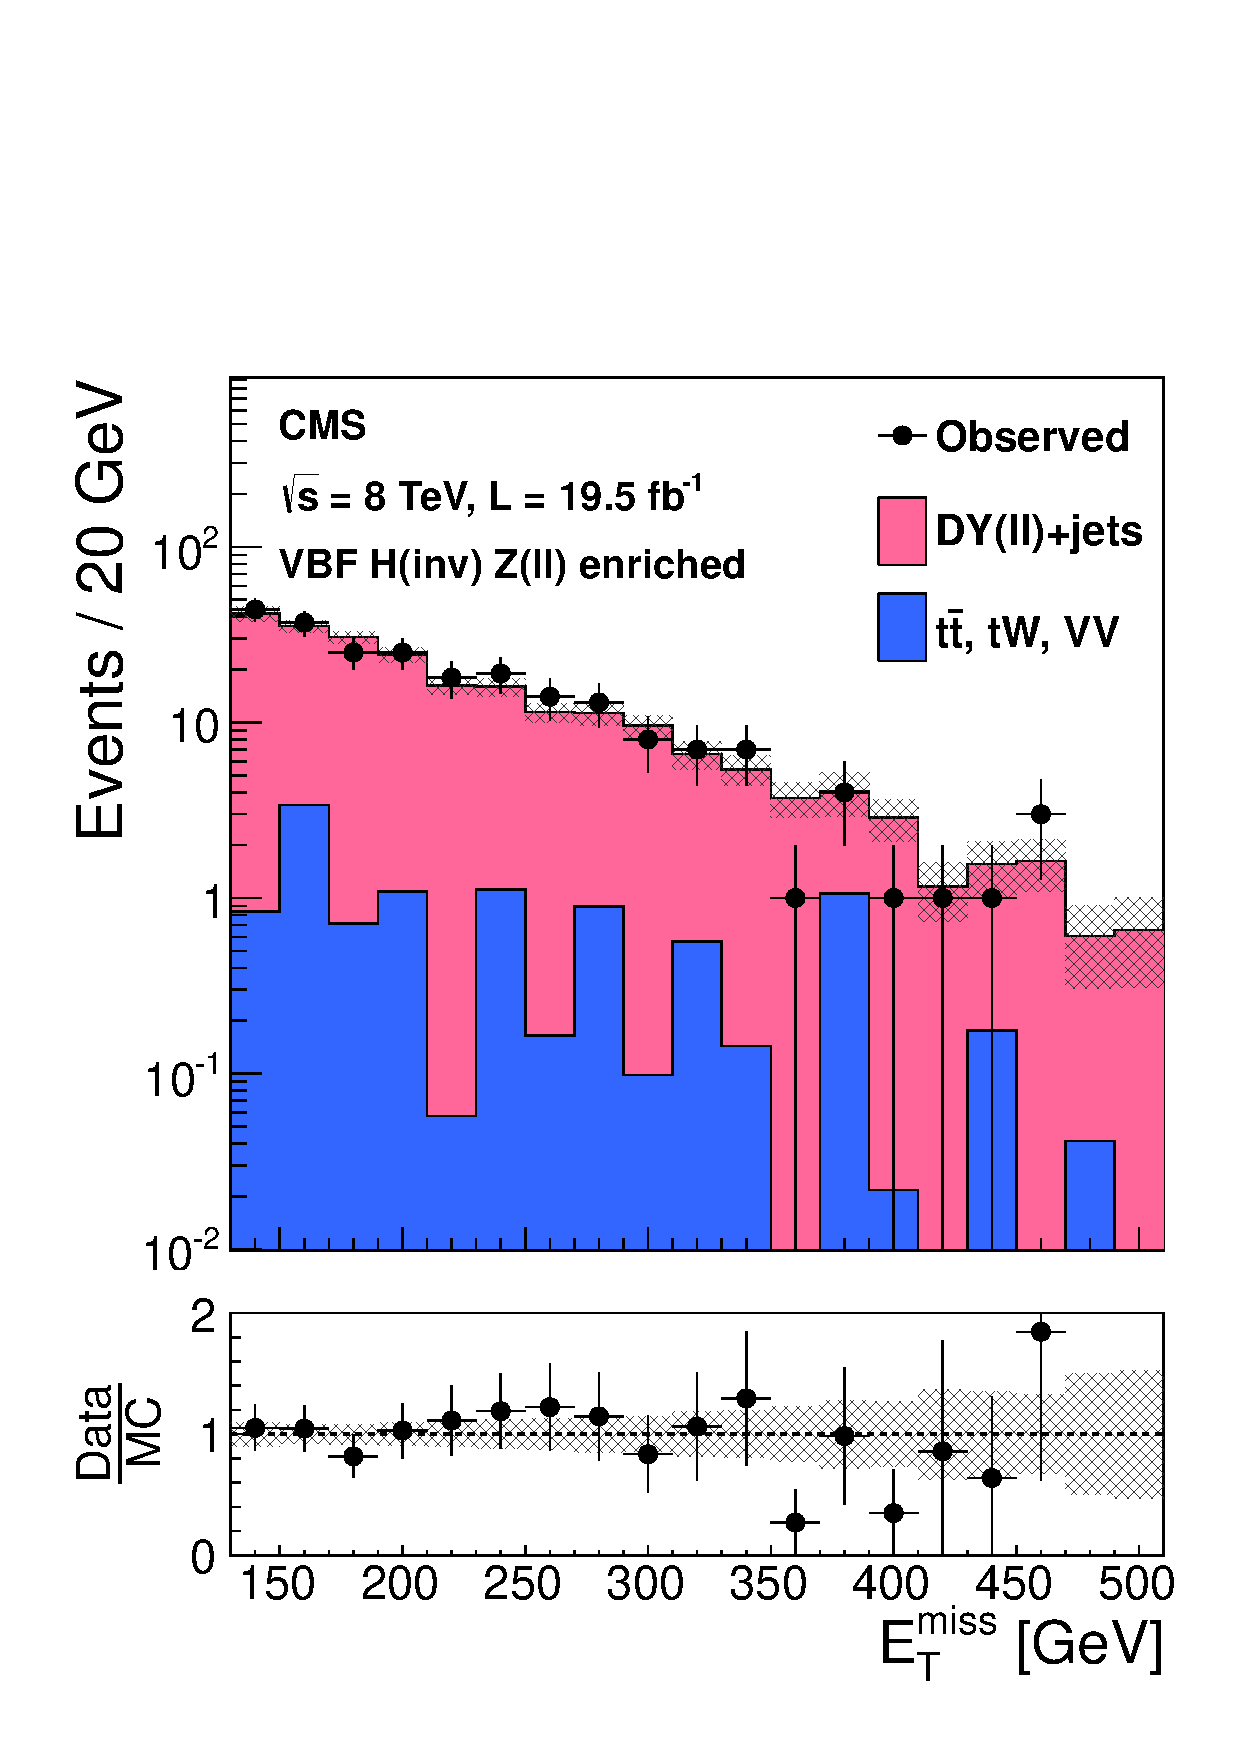
\includegraphics[width=.65\largefigwidth]{plots/prompt/VBF-ZCtrl-MET.pdf}}
  \subfloat[]{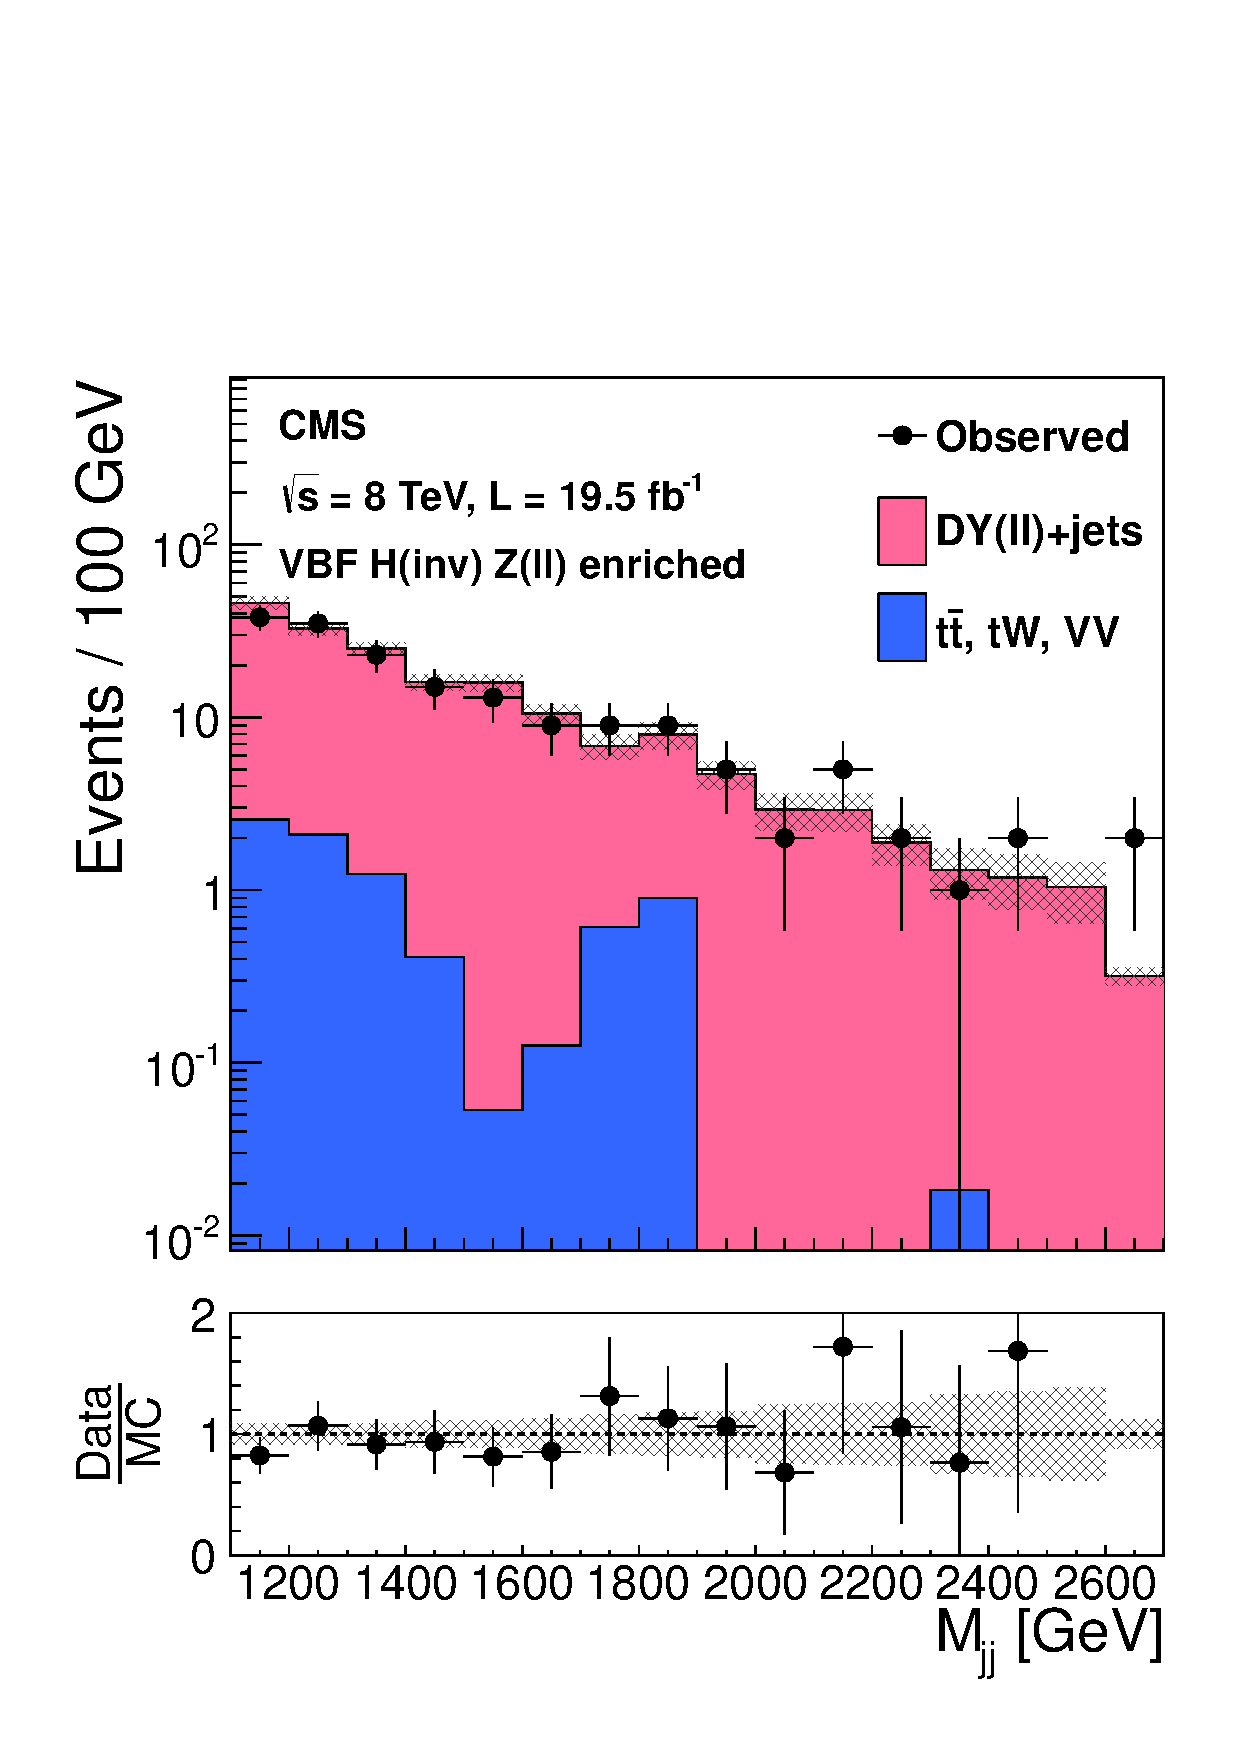
\includegraphics[width=.65\largefigwidth]{plots/prompt/VBF-ZCtrl-Mjj.pdf}}
  \caption{Distributions of the \METnoMU (a) and \Mjj (b) in a relaxed \PZ control region, with no requirement on \dphijj, the CJV removed, and the requirements on \Mjj and \detajj relaxed to 1000 \GeV and 3.5 respectively. DY(ll)+jets indicates the contribution from Z+jets processes and $t\bar{t}$, $t\PW$, VV indicates the contribution from minor backgrounds. The hatched region illustrates the systematic uncertainty~\cite{Chatrchyan:2014tja}.}
  \label{fig:promptznunu}
\end{figure}




\subsection{QCD}
\label{sec:promptacQCD}
The \ac{QCD} background remaining after the full event selection is mostly from events where jets are mismeasured. The size of the \ac{MC} samples available for studying this process is not sufficient for them to be relied upon for extrapolation from a control region to the signal region. The remaining \ac{QCD} background is therefore estimated using a so-called ``ABCD'' method. In this method four regions, A, B, C and D, are defined according to whether events pass or fail the \METnoMU and \ac{CJV} cuts, as shown in \FigureRef{fig:abcdmethod}. Region D is the signal region and regions A, B and C are three mutually exclusive control regions.

\begin{figure}
  \begin{tabular}{l|c|c|l}
    \multicolumn{1}{c}{}&\multicolumn{1}{c}{Fail \METnoMU} & \multicolumn{1}{c}{Pass \METnoMU} &\\
    \cline{2-3}
    Fail \ac{CJV} &\cellcolor{orange} A & \cellcolor{orange}B &\\
    \cline{2-3}
    Pass \ac{CJV} &\cellcolor{orange} C & \cellcolor{green}D &\\
    \cline{2-3}
  \end{tabular}

  \caption{A diagram of the regions used in the QCD ABCD background estimation method. Region D is the signal region and regions A, B and C are mutually exclusive control regions.}
  \label{fig:abcdmethod}
\end{figure}

The efficiency to pass the \METnoMU and \ac{CJV} cuts can be determined from the ratios between regions A and B, and A and C respectively. The number of events expected in the signal region is then:
\begin{align}
  \label{eq:abcd}
  \begin{split}
  N_{D}&=N_{A}\cdot\frac{N_{B}}{N_{A}}\cdot\frac{N_{C}}{N_{A}}\\
  &=\frac{N_{B}\cdot N_{C}}{N_{A}},
  \end{split}
\end{align}
where $N_{A,B,C}$ is the number of events observed in region $A,B,C$ in data minus the number expected from V+jets or other minor backgrounds, i.e. the number of events in the region believed to be from QCD. This method relies on the probability of an event passing the \ac{CJV} being uncorrelated with the \METnoMU of the event. This has been checked by comparing the \METnoMU distribution, below the 130 \GeV signal region requirement, for events which pass and fail the \ac{CJV} (see \FigureRef{prompt:qcdmetcjv}). The maximum fractional difference observed between bins of these two distributions is 40\%, so this is added as a systematic to the \ac{QCD} background yield. The method was also tested in a region orthogonal to the signal region with all requirements the same as those of the signal region except \dphijj which was required to be greater than 2.6. In this test region, which is expected to be \ac{QCD} dominated, the observation agreed with the expectation within 15\%, which is within the systematic uncertainty assigned to the method. The results of using this method to estimate the number of QCD events in the signal region are shown in \TableRef{tab:promptqcd}.

\begin{figure}
  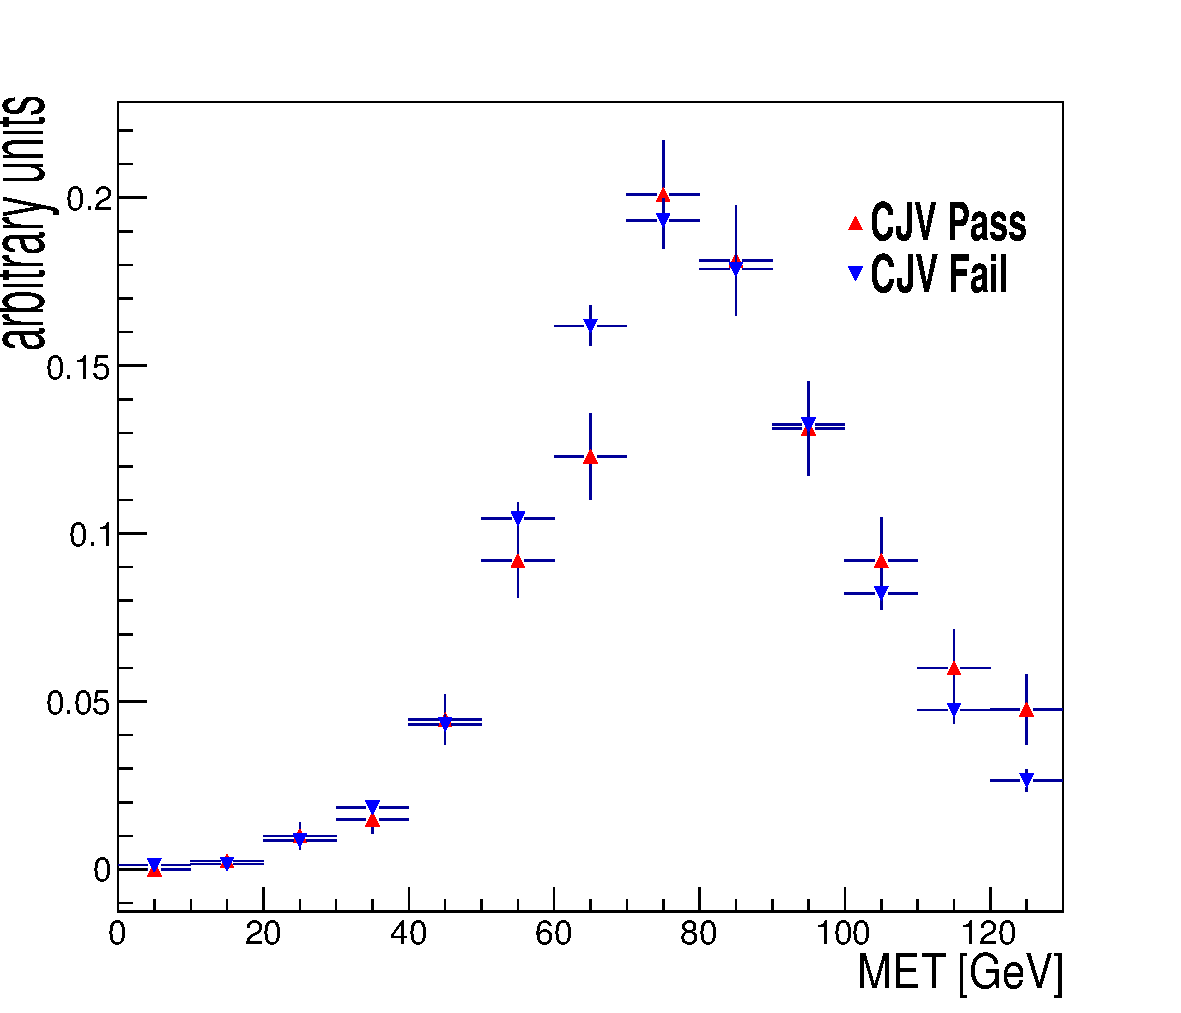
\includegraphics[width=1.2\largefigwidth]{plots/prompt/AN-12-403-figs/QCD3_CtrlLo_MET.pdf}
  \caption{Distribution of the \METnoMU for events passing and failing the CJV. Both distributions are normalised to a total integral of 1. The largest difference seen in any bin is 40\%. This difference is used to assign as a systematic uncertainty on the QCD background estimation.}
  \label{prompt:qcdmetcjv}
\end{figure}

%Table of results
\begin{table}
  \caption{Numbers of events from data and MC in each region used in the QCD background estimate and the final estimated number of events.}
  \label{tab:promptqcd}
  \begin{tabular}{lccc}
    \hline
    \hline
    Region & Data & Background & Data-Background \\
    \hline
    \hline
    $N_{A}$ & 5118 & $222\pm 14$ & $4896\pm 73$\\
    $N_{B}$ & 773  & $586\pm 17$ & $184 \pm 33$\\
    $N_{C}$ & 896  & $76.9\pm 8.3$ & $819\pm 31$\\
    \hline
    $N_{D}$ & - & - & \textcolor{red}{$30.9\pm 1.6$}\\
    \hline
    \hline
  \end{tabular}
\end{table}

\subsection{Minor backgrounds}
\label{sec:promptminor}
In addition to the V+jets and QCD backgrounds which account for 94\% of the expected events in the signal region, there is also a small number of events expected from other minor backgrounds including single top quark production, top quark pair production, diboson production and \Zmumu. Due to their small contributions these numbers of events are taken directly from \ac{MC}. The diboson backgrounds are simulated using \textsc{Pythia 6}, the single top quark background using \textsc{Powheg} and the top quark pair production and $\PZ/\gamma^{*}\rightarrow\ell\ell$ backgrounds using \textsc{MadGraph}. The cross-sections used to normalise these \ac{MC} samples were taken from the most up-to-date CMS published results at the time of the analysis~\cite{CMS:2012fza,CMS:2012iza,CMS:2012zva,CMS:2013qea,CMS:2013hea}. The final estimate of the number of events from minor backgrounds in the signal region is $20\pm 8.2$(MC stat), with 70\% of these expected to be from diboson production.


\section{Systematic uncertainties}
\label{sec:promptsyst}
The dominant uncertainties in the analysis are the statistical uncertainties on the V+jets backgrounds due to the number of data events observed in the control regions. In addition, as well as those mentioned in \SectionRef{sec:promptbkg}, there are several further systematic uncertainties on the expected numbers of signal and background events. These uncertainties are described individually below and the fractional uncertainty on the total expected number of signal and background events from all sources of uncertainty are summarised in \TableRef{tab:promptsysts}.
\subsection{Jet energy scale}
\label{sec:promptjes}
The reconstructed energy of a jet reconstructed by CMS is not necessarily the same as the true energy of all the particles that make it up. As described in \SectionRef{sec:jec}, jet corrections are applied to remedy this. The correction for the ratio between reconstructed and true jet energy is referred to as the \ac{JES}. Uncertainties on the \ac{JES} come from several sources. The \ac{JES} obtained from the dijet \pt balance method for instance has an uncertainty from the jet resolution bias~\cite{CMS-JME-10-011}. This bias arises because the jet \pt spectrum sharply falls with increasing \pt. Such a spectrum leads to the well measured jet being used as the base for the balance method being more likely to have fluctuated up in \pt than down. The main uncertainties in the photon/\PZ balance methods come from the limited number of events in the samples used. The \ac{JES} obtained in \ac{MC} is also different when measured with different \ac{MC} generators, which leads to an uncertainty.

These uncertainties on the \ac{JES} give rise to an uncertainty on the energy of all jets in CMS events. The impact of this uncertainty on the expected and observed event yields in this analysis was estimated by altering the \ac{JES} correction up by one standard deviation, ``JESUP'', and down by one standard deviation ``JESDOWN'', and recalculating the energy and momentum of all jets in each event. The \MET is recalculated taking into account the updated jet energies. Furthermore, as the jet energy scale uncertainty varies with \pt and $\eta$, it is possible for the \pt ordering of the jets to change when the \ac{JES} is changed. The \ac{VBF} tag pair is therefore chosen again, so as to be the new highest \pt pair of jets. 

After modifying the \ac{JES}, the analysis is performed again and the resulting change in the expected signal and background yields is taken to be the uncertainty due to the \ac{JES}. The sub-leading jet's \pt in a W+jets \ac{MC} sample is shown for the nominal \ac{JES}, JESUP and JESDOWN in \FigureRef{fig:promptjes}. It can be seen that altering the \ac{JES} results in a smooth change in the jet \pt, indicating that the difference in the number of events passing the analysis cuts is not due to individual events with large weights migrating in and out of the signal region.

%plot from AN-13-205
\begin{figure}
  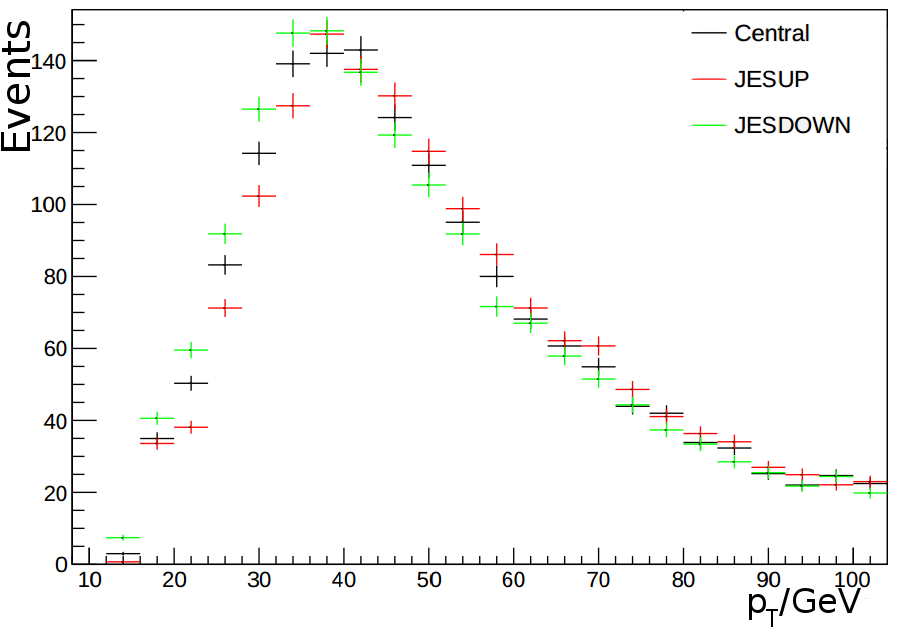
\includegraphics[width=\largefigwidth]{plots/prompt/jescheckzoom.png}
  \caption{The distribution of the sub-leading jet's \pt in W+Jets MC events with the nominal JES and for JESUP and JESDOWN.}
  \label{fig:promptjes}
\end{figure}

\subsection{Jet energy resolution}
\label{sec:promptjer}
The width of the jet energy distribution, the \ac{JER}, differs between \ac{MC} and data. This is partly due to \ac{MC} samples being generated before and during data taking, and thus before a measurement of the exact resolution in data can be performed. Measuring the \ac{JER} in data is done in a very similar way to the measurement of the \ac{JES} using dijet and photon/\PZ-jet balance techniques and by comparing the reconstructed energy to that generated in \ac{MC}, and thus has the same sources of uncertainty.

To correct the \ac{MC} resolution to match that in the data, the \pt of all jets in \ac{MC} is ``smeared''. The smearing is carried out using two methods. The first method is used for jets in \ac{MC} that are within 0.5 in the $\eta-\phi$ plane of a generator jet. In this method the difference between the reconstructed and generator jet \pt is scaled by a correction factor, $c$, chosen to be the ratio between the resolution of the data and \ac{MC} and calculated as a function of the jet's \pt and $\eta$. The resulting jet \pt is given by:
\begin{equation}
  \label{eq:promptjermatched}
  \pt'=\rm{max}\left[0,\mathnormal{p}_{{\mathrm{T}}gen}+\mathit{c}\left(\mathnormal{p}_{\mathrm{T}}-\mathnormal{p}_{{\mathrm{T}}gen}\right)\right],
\end{equation}
where \pt is the initial transverse momentum, $\pt'$ is the transverse momentum after smearing and $p_{\mathrm{T}gen}$ is the matched generator jet's \pt. This procedure has the advantage that the smearing is not reliant on random factors and is therefore reproducible, making synchronisation between analysis implementations easier. The factor $c$ depends on the \pt and $\eta$ of the jet and is calculated so as to represent the average resolution over the whole 2012 run period. 

The second method is used when a jet has no matching generator jet. In this case a random correction is necessary. The technique used is to add a fluctuation to the jet's \pt with a size obtained by sampling a gaussian with width:
\begin{equation}
  \label{eq:promptjerunmatched}
  \sqrt{\left(c^{2}-1\right)\sigma_{MC}},
\end{equation}
where $c$ is the same correction factor from the method above and $\sigma_{MC}$ is the initial \ac{MC} resolution as a function of \pt and $\eta$. $\sigma_{MC}$ was measured by performing a gaussian fit to the distribution of the ratio between the generator-level and offline jet \pt observed in $\PW+$jets \ac{MC}. As well as being random and thus difficult to reproduce, this method has the disadvantage that it can only be used to worsen the resolution. 

The analysis is performed three times with three different smearings, one where the MC resolution is smeared to match the nominal data resolution, which is used for the main signal and background estimations, and two where the \ac{MC} resolution is made to match the improvement, ``JERBETTER'' and worsening, ``JERWORSE'' of the jet energy resolution by one standard deviation. For the nominal resolution $c-1$ varies from less than 1\% in the central region, to 9\% in the \ac{HF}, while for ``JERBETTER'' and ``JERWORSE'' it varies from 10\% in the central region of the detector to 49\% in the \ac{HF}. In the case of the nominal and JERWORSE smearings the limitation that the unmatched jet smearing method can only worsen the resolution is not a problem, as the initial \ac{MC} resolution is better than that in data for all values of jet \pt and $\eta$. However, for the JERBETTER smearing it is necessary to improve the resolution for some jets. Fortunately, the differences between the generated resolution and the JERBETTER resolutions where improved resolution is required are small, so in these cases no smearing is applied. For all smearings the resulting changes in jet \pt are propagated through to the \MET. The differences between the signal and background yields obtained with the nominal \ac{JER}, JERBETTER and JERWORSE are used to assign an uncertainty due to the \ac{JER}.

\subsection{Unclustered energy scale}
\label{sec:promptues}
In addition to the uncertainties on the \MET from the propagation of \ac{JES} and \ac{JER} uncertainties there are also uncertainties from the other elements contributing to the \MET. Electrons and muons contribute to the \MET, but have very good resolution and small scale uncertainties compared to jets so their contribution to the \MET uncertainty is considered negligible~\cite{CMS-PAS-JME-12-002}. Unclustered energy, which is made up of all of the energy deposits in the calorimeters not identified as part of an object, such as a jet or lepton, still contributes to the \MET, and has a non-negligible scale uncertainty~\cite{CMS-PAS-JME-12-002}. %citation

The \ac{UES} is measured using photon and \PZ events with jets present in them, where it can be assumed that the \MET should be zero~\cite{CMS-PAS-JME-12-002}. After jet energy corrections, the distribution of the remaining difference between the photon or \PZ momentum and the jets is therefore centered around zero, and its width can be taken as the uncertainty on the \ac{UES}. The \ac{UES} in all events is modified up and down by this uncertainty and the \MET recalculated. The differences in the obtained signal and background event yields obtained through this process are used as the uncertainty from this source.

\subsection{Lepton identification and isolation efficiency}
\label{sec:promptlepweights}
As described in \SectionRef{sec:mcweights} \ac{MC} events are reweighted using scale factors to account for differences in the electron and muon identification and isolation efficiency. The weights due to these efficiencies are varied up and down by the uncertainties from the tag and probe method used to measure them, and the difference in the resulting signal and background yield used as the uncertainty from this source.

An uncertainty of 8\% is added to the estimate of the $\PW\rightarrow\tau\nu$ background to account for the uncertainty in the tau identification efficiency, which is measured using $\PZ\rightarrow\tau\tau$ events where one tau decays to a muon and the other hadronically~\cite{Chatrchyan:1385560}. 5\% of events in the $\PW\rightarrow\tau\nu$ control region also appear to be due to $\PW\rightarrow e\nu$ events where the electron or a jet has been misreconstructed as a tau, so a further 5\% systematic is assigned to the $\PW\rightarrow\tau\nu$ estimate.


\subsection{Other uncertainties}
\label{sec:promptzextrap}
Additional uncertainties arise from several sources. For instance, the \Znunu background estimate is reliant on the ratio of the cross-sections for the \Znunu and \Zmumu processes in the phase space of this analysis. A 20\% uncertainty on this ratio was applied to cover the difference between the values of the ratio calculated using \textsc{MadGraph} and using \textsc{MCFM}~\cite{ARTICLE:CMSAN-12-403}. Further uncertainties come from the measurement of the distribution of the number of primary vertices used in the pileup weights, described in \SectionRef{sec:mcweights}, the \ac{PDF}s and \ac{QCD} scale used in the signal cross-section measurements~\cite{Dittmaier:2011ti,Dittmaier:2012vm}, differences in the \ac{ggH} \dphijj spectrum depending on the \ac{MC} generator used~\cite{ARTICLE:CMSAN-12-403}, the cross-sections used to normalise the minor backgrounds, described in \SectionRef{sec:promptminor}, and the measurement of the total integrated luminosity~\cite{CMS-PAS-LUM-13-001}.


\begin{table}
  \caption{A summary of the uncertainties in the total expected signal and background yields. All uncertainties are quoted as the percentage change in the yield when each effect is varied up and down according to its uncertainty. The signal yields assume a Higgs boson mass of 125\GeV.}
  \label{tab:promptsysts}
  \begin{tabular}{lcc}
    \hline
    \hline
    Uncertainty source & Total background & Signal \\
    \hline
    Control region statistics               & 11\%          & \NA  \\
    MC statistics and \Znunu cross-section ratio  & 11\%          & 4\%  \\
    \ac{JES}, \ac{JER} and \ac{UES}         & 7\%           & 13\% \\
    QCD background estimation               & 4\%           & \NA  \\
    Lepton efficiency                       & 2\%           & \NA  \\
    Luminosity                              & 0.2\%         & 2.6\%\\
    Cross-sections                          & 0.5--1\%      & \NA  \\
    PDFs                                    & \NA           & 5\%  \\
    \ac{QCD} scale     & \NA           & 4\%  \\
    \ac{ggH} \dphijj spectrum           & \NA           & 4\%  \\
    \hline
    Total & 18\% & 14\% \\
    \hline
    \hline
  \end{tabular}
\end{table}

\section{Results}
\label{sec:promptresults}
The final results of all the background estimation methods and systematic uncertainty studies are summarised in \TableRef{tab:promptresults}. The total number of events expected from background processes in the signal region is $332\pm 46\stat\pm 45\syst$. The presence of a Higgs boson with a mass of 125 \GeV, \ac{SM} production and \BRinv$=100\%$ would be expected to yield $224\pm 31$  signal events, with 6\% of these from \ac{ggH} and the remainder from \ac{VBF} production. 390 events are observed, which is within one standard deviation of the background-only prediction. \FigureRef{fig:promptresults} shows the \METnoMU and \Mjj of the background and signal events expected, and the data observed, in the signal region. 

%table of yields
\begin{table}
  \caption{The estimated numbers of background and signal events, together with the observed yield, in the signal region. The signal yield assumes a Higgs boson mass of 125 \GeV and \BRinv$=100\%$.}
  \label{tab:promptresults}
  \begin{tabular}{lc}
    \hline
    \hline
    Process & Event yield \\
    \hline
    \hline
    \Znunu & $99\pm 29\stat\pm 25\syst$ \\
    $\PW\rightarrow e\nu$ & $67\pm 5\stat\pm 16\syst$ \\
    $\PW\rightarrow\mu\nu$ & $63\pm 9\stat\pm 18\syst$ \\
    $\PW\rightarrow\tau\nu$ & $53\pm 18\stat\pm 18\syst$ \\
    QCD multijet & $31\pm 5\stat\pm 23\syst$ \\
    Minor backgrounds & $20\pm 8\syst$\\
    \hline 
    Total background & $332\pm 36\stat\pm 45\syst$ \\
    \hline
    \ac{VBF} H(inv.) & $210\pm 29\syst$ \\
    \ac{ggH}(inv.) & $14\pm 10\syst$ \\
    \hline 
    \hline
    Observed data & $390$ \\
    \hline
  \end{tabular}
\end{table}

%distributions
\begin{figure}
  \subfloat[]{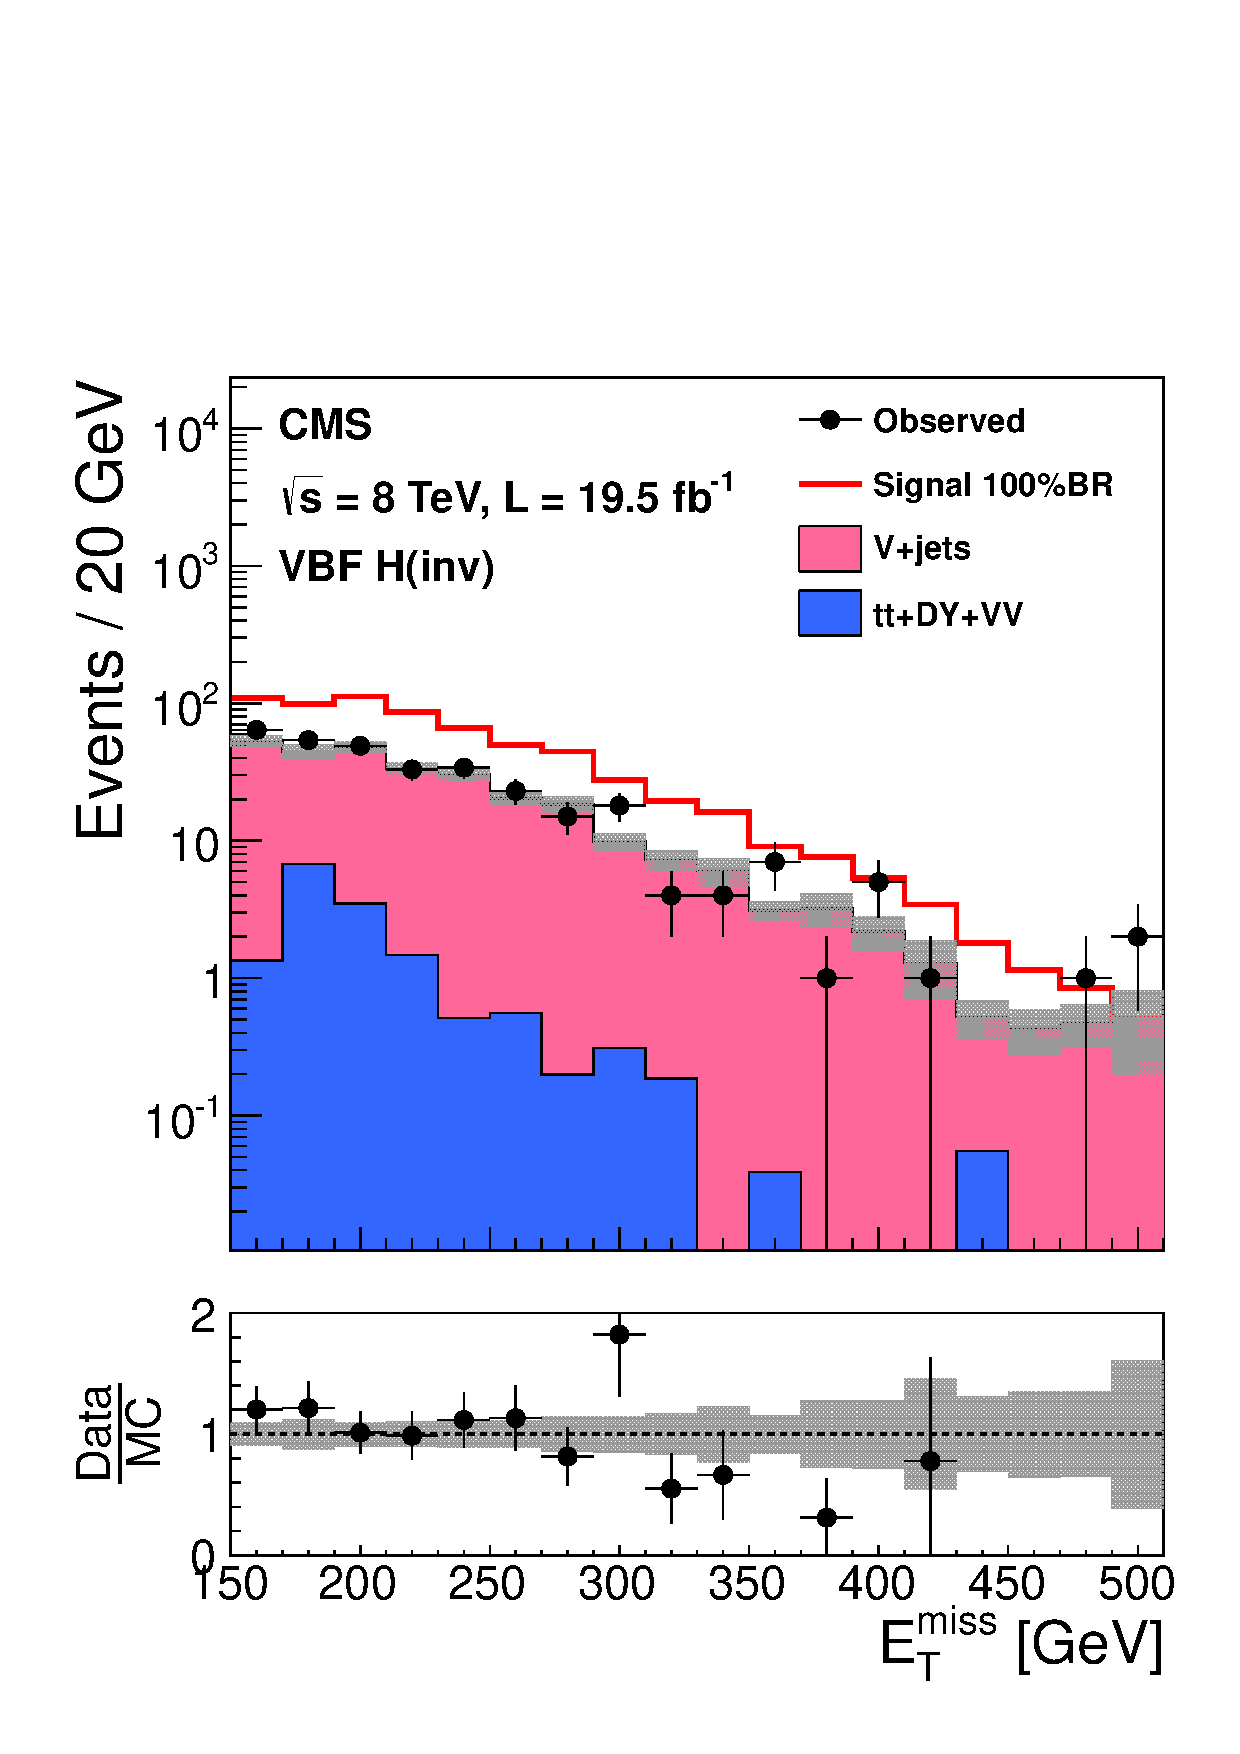
\includegraphics[width=.65\largefigwidth]{plots/prompt/AN-12-403-figs/SignalRegionMET.pdf}}
  \subfloat[]{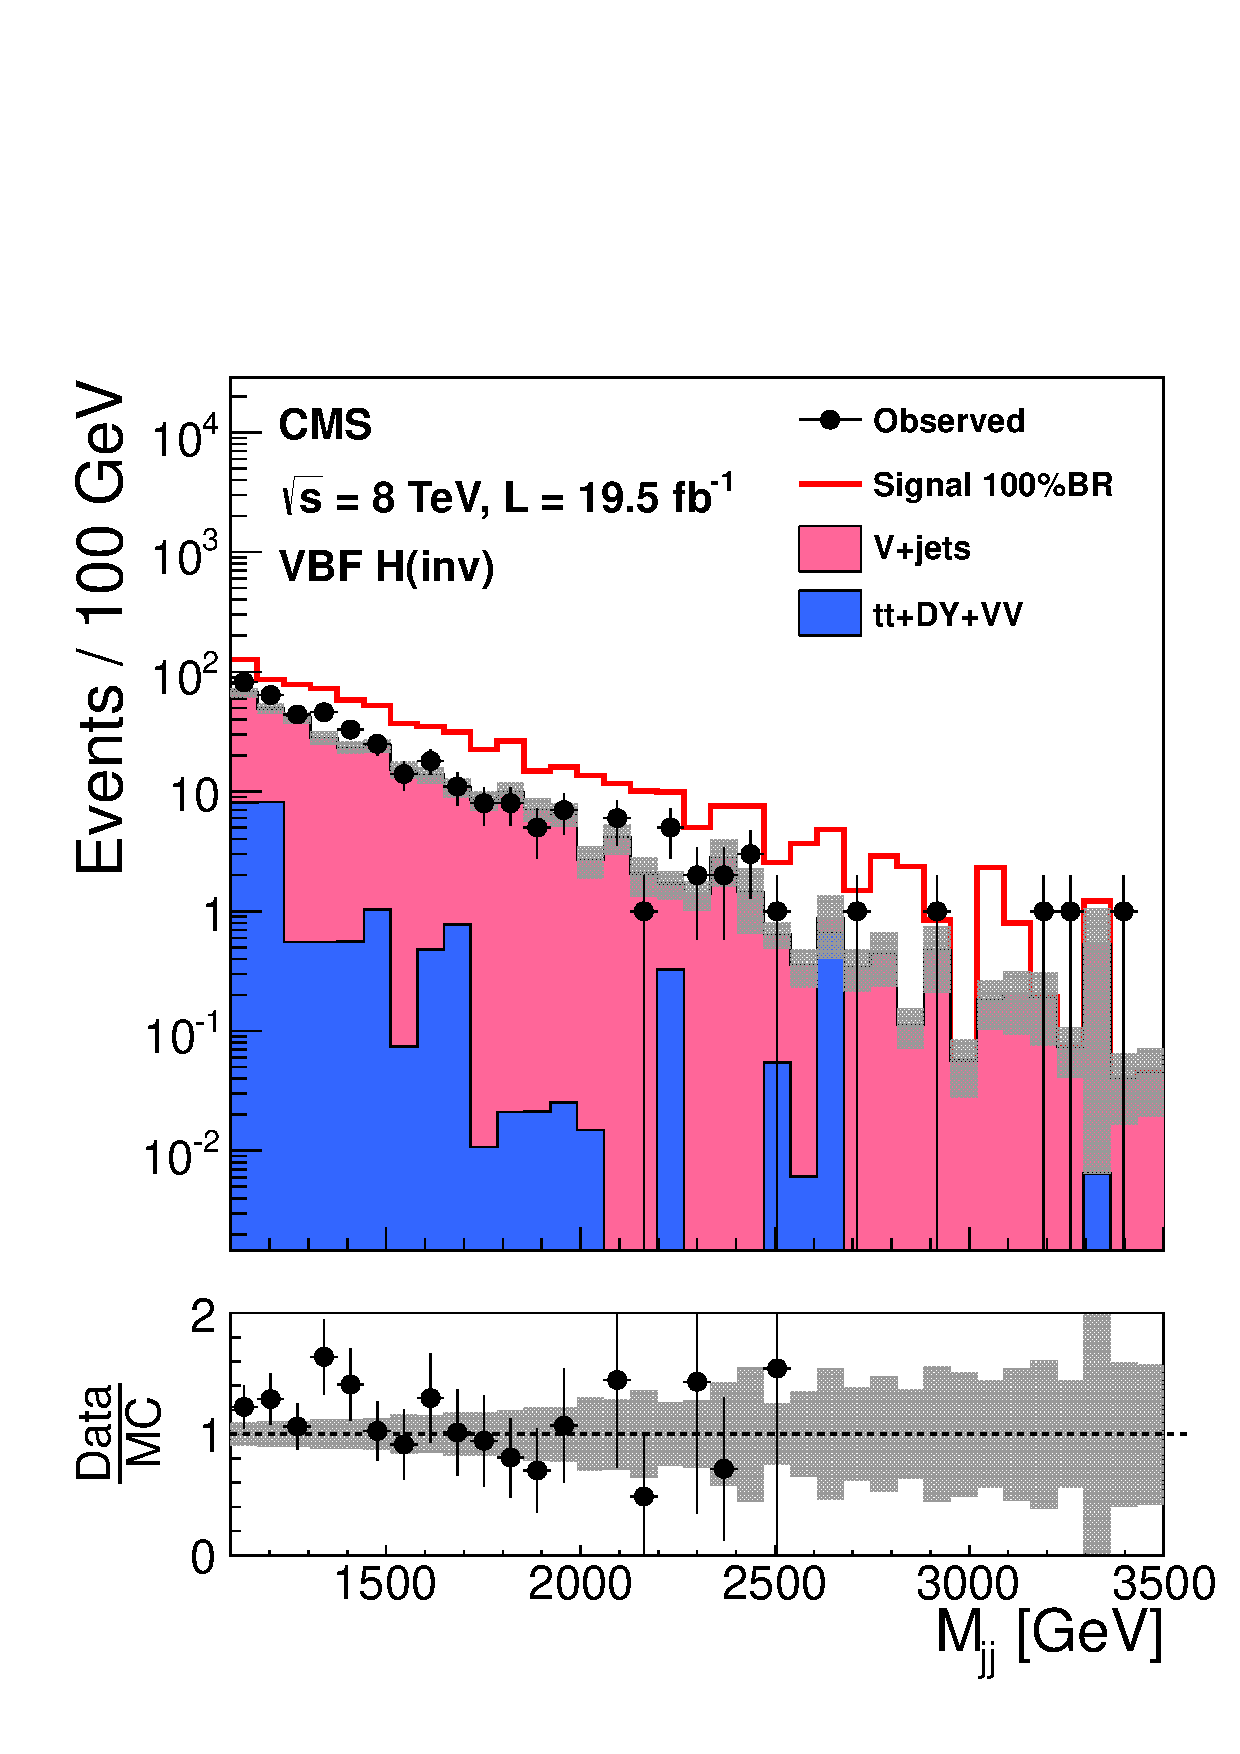
\includegraphics[width=.65\largefigwidth]{plots/prompt/AN-12-403-figs/SignalRegionMjj.pdf}}
  \caption{Distributions of the \METnoMU (a) and \Mjj (b) of events observed in data and expected from the background estimation methods described in \SectionRef{sec:promptbkg} in the signal region. tt+DY+VV indicates the contribution from minor backgrounds. The hatched region illustrates the systematic uncertainty. The QCD background is not shown due to the very low number of events in the MC samples. The cumulative effect of a signal from a Higgs boson with mass of 125 \GeV, decaying 100\% to invisible final states is also shown~\cite{Chatrchyan:2014tja}.}
  \label{fig:promptresults}
\end{figure}

As no excess is observed, the asymptotic $CL_{S}$ technique, described in \SectionRef{sec:stats}, is used to place an upper limit on the production cross-section times branching fraction, $\sigma\times\mathcal{B}$, at 95\% \ac{CL}. Under the assumption of \ac{SM} production this limit can be interpreted as a limit on \BRinv. All systematic uncertainties are modelled as log-normally distributed nuisance parameters, with the exception of the statistical uncertainty on the $Z\rightarrow\nu\nu$ background, which is modelled as a gamma-normally distributed nuisance due to the low number of events in the dimuon control region. A gamma-normal distribution is used in the case of control regions with low numbers of events because in this case the central limit theorem does not apply so the Poisson probability of observing a certain number of events is very asymmetric; this asymmetry is well modelled by a gamma-normal distribution~\cite{2003sppp.conf...35L}.

The resulting upper limits are shown as a function of Higgs boson mass in \FigureRef{fig:promptlimits}, with the 95\% \ac{CL} observed (expected) limit on \BRinv for a 125 \GeV Higgs boson being 65\% (49\%). The green and yellow bands shown in \FigureRef{fig:promptlimits} denote the one and two sigma uncertainty bands respectively of the expected limit, also calculated using the asymptotic technique. The one (two) sigma band represents the region that the observation is expected to lie in 68\% (95\%) of the time if the background-only hypothesis is true.

This was the first published search for invisibly decaying Higgs bosons in the \ac{VBF} channel. It can be seen that for all values of Higgs boson mass investigated the observed limit is approximately one sigma above the expected limit. If the measurements of the limit at each Higgs boson mass were not correlated, this could be seen as evidence for an excess. However, as this analysis has only a single bin, and no information on the shape of the event variable distributions is used, the measurements for the different Higgs boson masses are 100\% correlated with each other. The analysis therefore sees no significant evidence of non-\ac{SM} behaviour.

%limit plots
\begin{figure}
  \subfloat[]{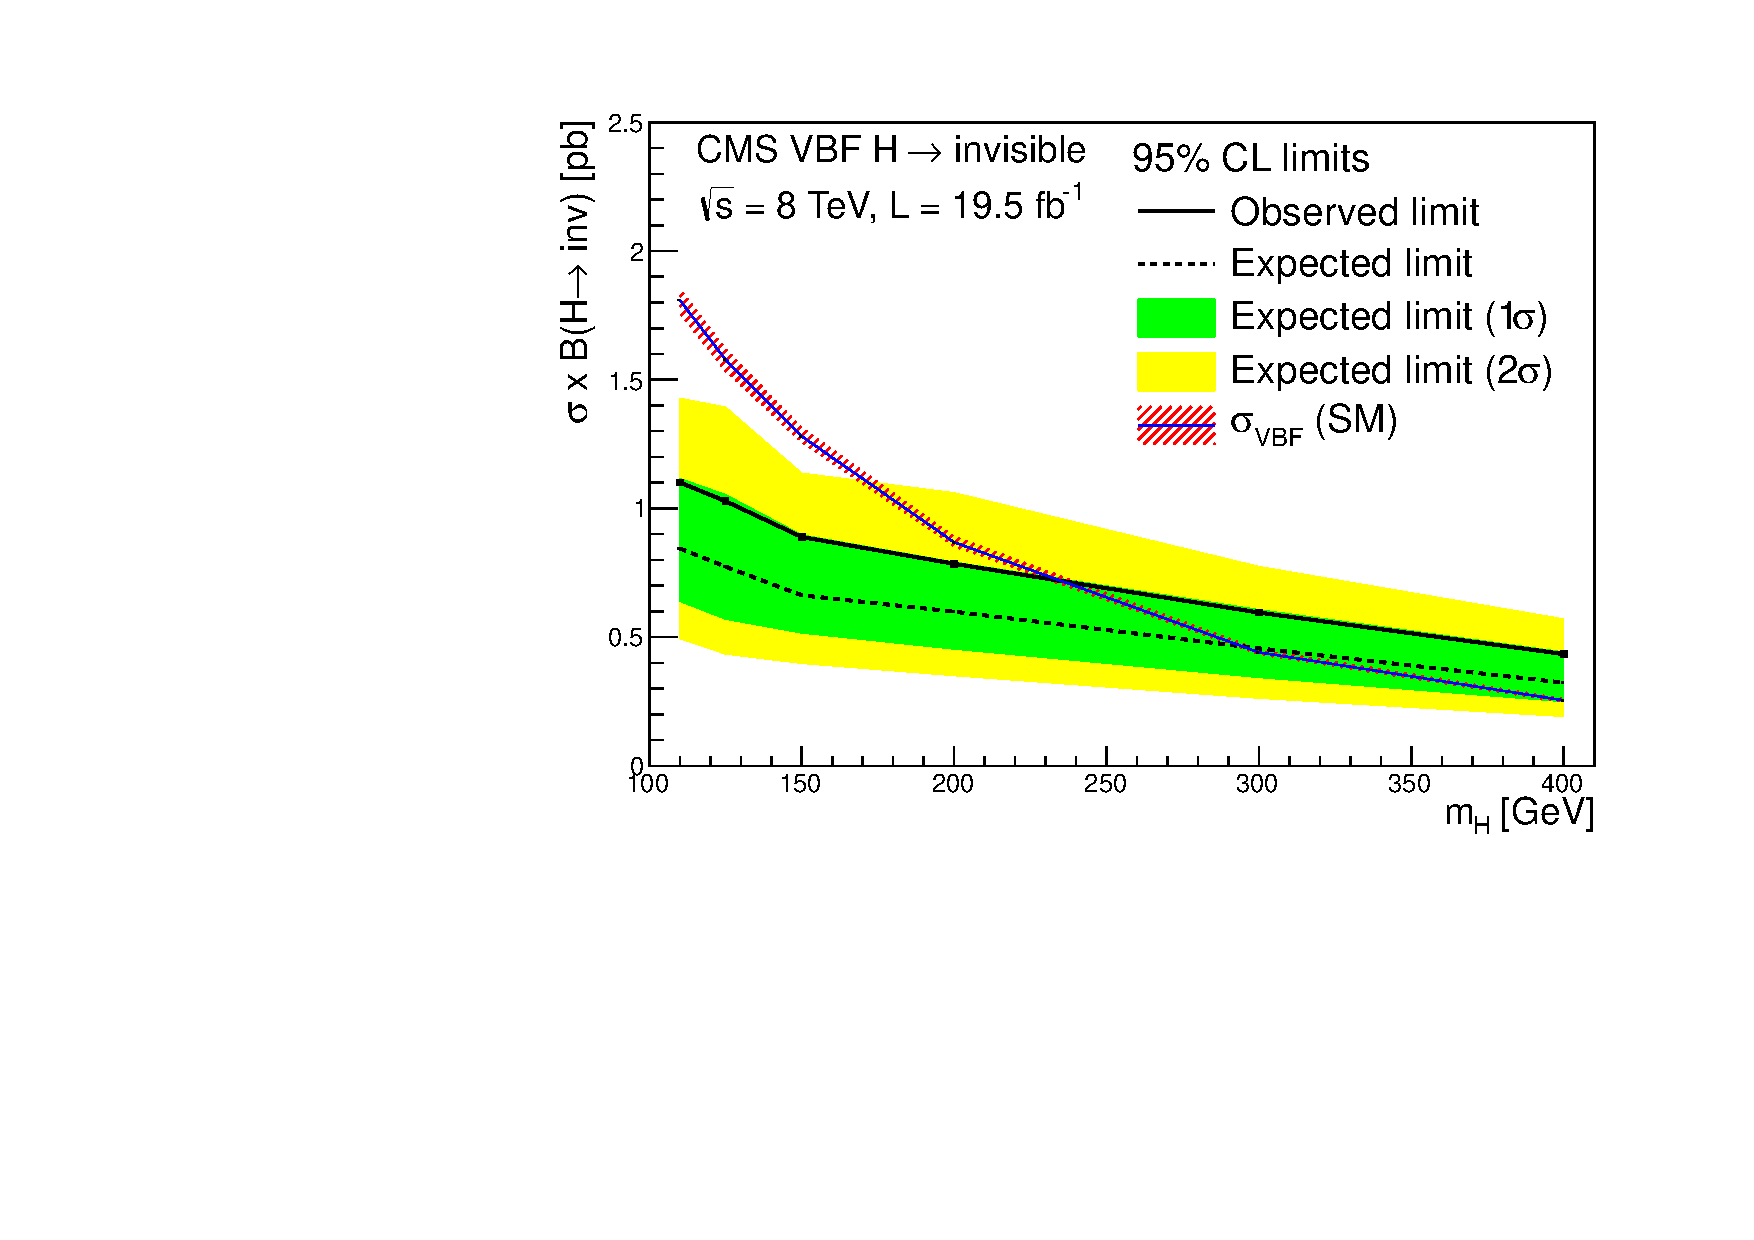
\includegraphics[width=\largefigwidth]{plots/prompt/HIG-13-30-figs/vbfxslimit.pdf}}

  \subfloat[]{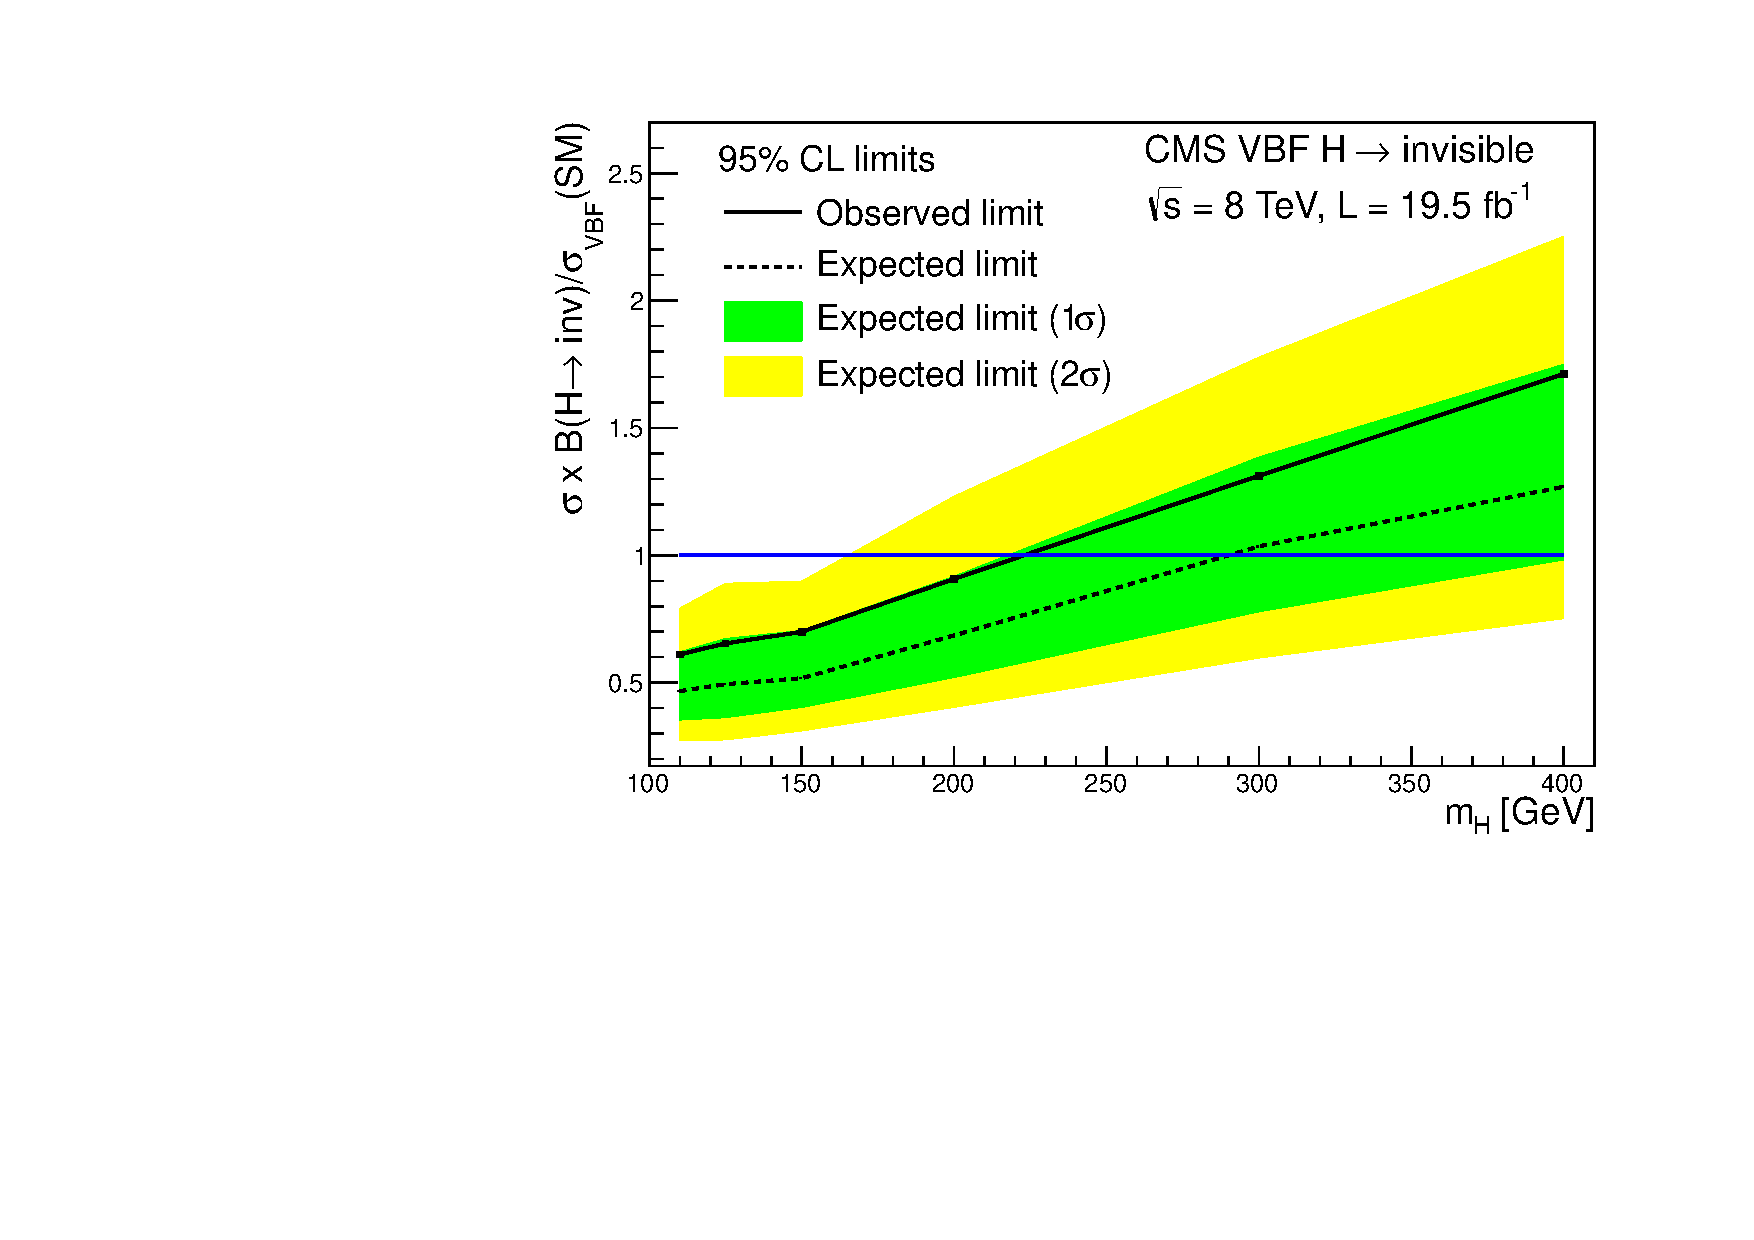
\includegraphics[width=\largefigwidth]{plots/prompt/HIG-13-30-figs/vbflimit.pdf}}
  \caption{Expected and observed 95\% CL upper limits on the VBF $\sigma\times\mathcal{B}$ in \pb (a) and normalised to the SM VBF Higgs boson production cross-section (b)~\cite{Chatrchyan:2014tja}. The green and yellow bands indicate the 68\% and 95\% confidence intervals on the expected limit respectively.}
  \label{fig:promptlimits}
\end{figure}
